\chapter{Related Work}
In this section I will describe the most relevant works that inspired this work  or are linked to a specific topic. The aim of this section is to provide a basis for both, the benchmarking model that is developed in section \ref{ch:benchmark}, and the capacitive proximity sensing prototypes described in section \ref{ch:proto}. The related works are distinguished into four distinct parts. At first I will give a general introduction to electric field sensing, including a discussion on different properties, physical background, the influence of materials and geometry and different data processing methods. Afterwards I will  present relevant applications using capacitive proximity sensing, ranging from historical works to very recent systems. In the next section various sensing technologies are introduced that are used in smart environment systems. Finally I will identify and group different applications in smart environments, providing a basis for the benchmarking model.
\section{Electric field sensing}
Any electric charge is applying an attracting or repelling force to other charged particles in space. This force has a distinct magnitude and direction for any point in space and thus creates an electric field. The presence of conductive objects is modifying the properties this field. Thus, in its most basic definition electric field sensing allows us to gather information about the field properties at a certain point in space. If we continuously monitor the field we are able to measure the disturbance and associate it to objects that are passing through, allowing to gather information about their specific properties. In this section we will give a brief overview of the development of electric field sensing technology, the physical background, different measuring modes and how to process data acquired by digital sensor devices.
\subsection{A brief history of capacitive proximity sensing}
\begin{figure}[h]
\centering
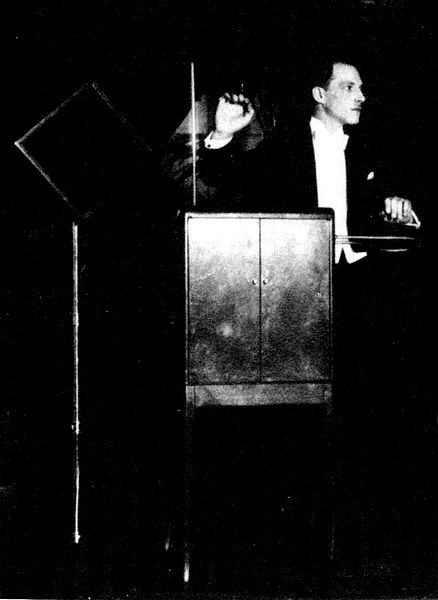
\includegraphics[width=0.4\textwidth]{images/leon_theremin.jpg}
\caption{Leon Theremin playing his epnoymous electronic musical instrument \cite{Glinsky2000}}
\label{fig:leon_theremin}
\end{figure}
In the last decades of the 19th and the beginning of the 20th century a considerable number of inventors and scientists performed research on the application of electric systems, sparking innovations such as electric lighting, electric motors, telegraphy and radio communication. Lev Sergeyevich Termen or Léon Theremin in the American naming was a Russian inventor most famous for designing the theremin. This early electronic musical instrument could be played without touch. One hand is controlling the pitch and the other the volume by changing the distance to an antenna. Initially designed as a motion detector, this device is transferring the influence of the human body on an oscillating electric field to an audible sound \cite{Glinsky2000}. 

Electric field imaging was a research focus at the MIT in the 1990s. A research group in the Media Lab division including Joseph A. Paradiso, Thomas G. Zimmerman, Joshua R. Smith designed various sensing devices and evaluated various applications in HCI \cite{Zimmerman1995}\cite{Smith1999a}.
\subsection{Physical properties}
A complete overview about the electrostatic principles of capacitive proximity sensing can be found in the book by Baxter \cite{Baxter1996}, chapters 2 and 6. We will give a very brief introduction to this topic in the following section.
\begin{figure}[h]
\centering
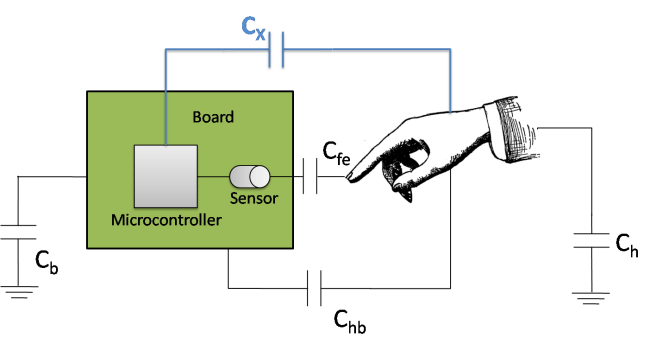
\includegraphics[width=0.4\textwidth]{images/cap_blackbox.png}
\caption{Black box setup of a capacitive proximity sensor}
\label{fig:cap_blackbox}
\end{figure}
The basic setup of a typically used sensor is shown in Figure \ref{fig:cap_blackbox}. The proximity capacitance \(C_{x}\) can be determined using a combination of serial and parallel circuits of capacitors, resulting in the following equation:
\begin{equation}
C_{x}=\left(\left(C_{hb}+\frac{C_{h}C_{b}}{C_{h}+C_{b}}\right)^{-1}\frac{1}{C_{fe}}\right)^{-1}
\end{equation}
Additionally there are parasitic capacitance components, i.e. disturbing capacitance values within the system. Sources are:
\begin{itemize}
\item Sensing electrode capacitance
\item Capacitance between sensing electrode and ground plane
\item Intercapacitance between neighboring traces on the board
\end{itemize}
The present parasitic capacitances \(C_{par}\) amount to values approximately between \(10pF\) and \(300pF\) and are therefore considerably larger than the value of the proximity capacitance \(Cx\), being between \(0.1pF\) and \(10pF\). The total capacitance sensed is the sum of parasitic and proximity components. 
\begin{equation}
C_{S}=C_{X}+C_{par}
\end{equation}

It is obvious that this parasitic capacitance is considerably higher than the capacitance induced by an approaching object. However, this parasitic capacitance is typically static and can therefore be calibrated in a way not affecting the measurement. 
\begin{figure}[h]
\centering
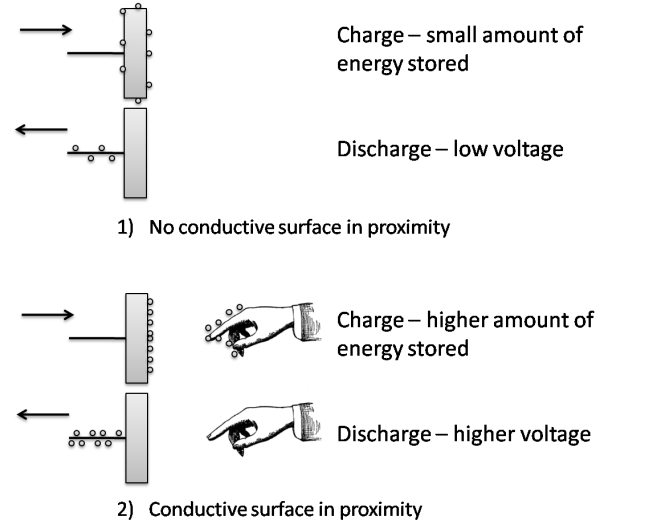
\includegraphics[width=0.4\textwidth]{images/cap_procedure.png}
\caption{Capacitive sensing procedure}
\label{fig:cap_procedure}
\end{figure} 
Now we will shortly discuss how we can estimate the capacitance of common objects that approach the sensor. Any object exhibits capacitance in respect to infinity. Surveying simple geometric shapes this capacitance is analytically determinable, e.g.:
\begin{equation}
C=8\epsilon_{0}r Disk
\end{equation}
\begin{equation}
C=4\pi\epsilon_{0}r	Sphere
\end{equation}

\(\epsilon_{0}\) is the vacuum permittivity and \(r\) the respective radius. This free space capacitance is increasing as soon as another object is approaching, caused by the capacitance of this second object, resulting in mutual capacitance. Looking at generic formulas, determining capacitance between parallel plates this behavior can be described analytically.
\begin{align}
C&=\frac{Q}{V} & C&=\epsilon_{0}\epsilon_{r}\frac{A}{d}
\end{align}
The capacitance is directly proportional to the plate area \(A\) and inversely proportional to the distance d between the plates, with \(\epsilon_{r}\) being the relative static permittivity of the dielectric between the plates. Sensor electronics are grounded with the body acting as ground itself. The sensor plate is continuously charged using a constant voltage \(V\). A higher capacitance allows the system to hold a larger charge. If the system is connected to the ground, the sensor capacitor is discharged through a resistor. The resulting voltage is depending on the available charge, shown in the equation above. Furthermore the required time to discharge the capacitor is increased. This process is symbolized in Figure \ref{fig:cap_procedure}.

\subsection{Proximity sensing versus touch sensing}
\begin{figure}[h]
\centering
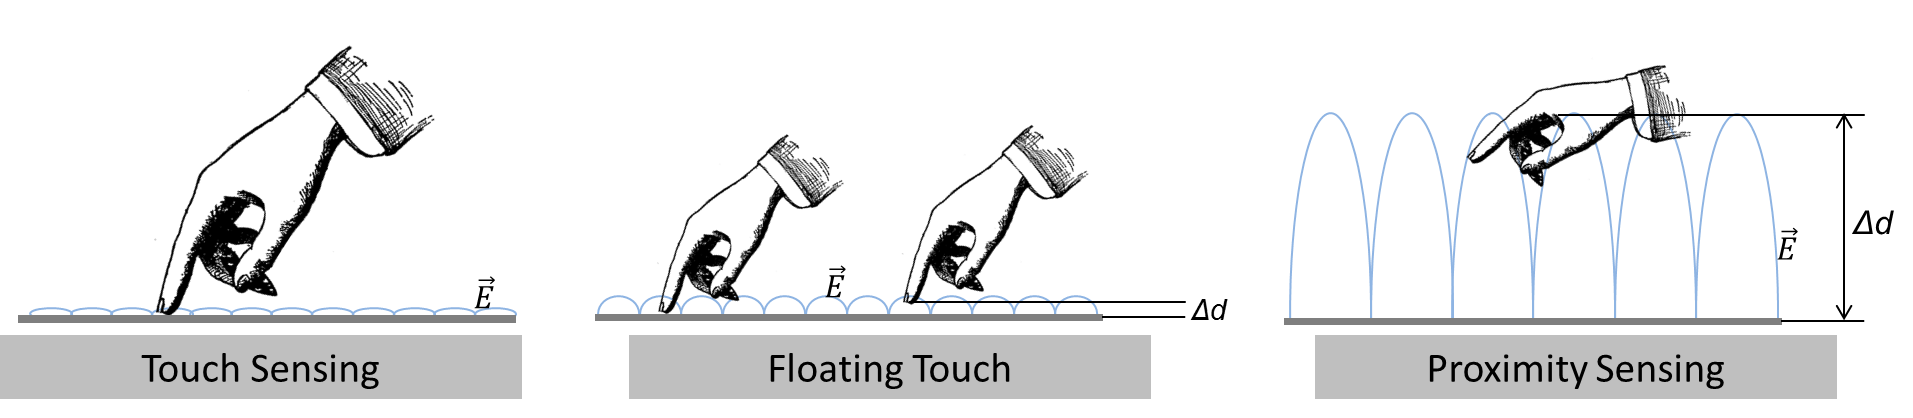
\includegraphics[width=1.0\textwidth]{images/cap_projected_sensing_methods.png}
\caption{Different projected capacitive sensing methods based on distance}
\label{fig:cap_proj_sensing_methods}
\end{figure} 
The most ubiquitous usage of capacitive sensing technology can be found in touch screens. As the trend went from pen-controlled mobile systems to finger controlled devices with the first iPhone in 2007, projected capacitance touch is the most prevalent technology for touch screens. It uses various layers of transparent electrodes or nanowires to detect the mutual capacitance as objects enter the detection area \cite{Barrett2010}. The commercially available devices have gained additional abilities over the last few years, leading to the development of “floating touch” systems that are able to track fingers in gloves or fingers that are hovering above the surface \cite{Cypress2012, Nokia2012}. Applications are the usage of mobile devices in cold outdoor temperatures or additional navigation fea-tures based on the hovering fingers. In consequence we can distinguish the three different projected capacitive sensing methods as shown in Figure \ref{fig:cap_proj_sensing_methods}:
\begin{itemize}
\item Touch sensing - densely distributed sensors are tuned to project a weak electric field in order to detect one or more objects touching the interactive surface. The sensors have to be close to the surface.
\item Floating touch - densely distributed high-sensitivity sensors are able to detect both touches and very near objects (\(<2cm\)) to enable usage using protective gear or additional navigation feature. The sensors have to be close to the surface.
\item Proximity sensing - sparsely distributed sensors create a stronger electric field that propagates into space in order to detect larger objects, such as hands, that are in proximity of the interactive surface. Achievable distances are up to 30 centimeters and the sensors may be applied below thick non-conductive material.
\end{itemize}
\subsection{Measuring modes}
\begin{figure} [h]
\centering
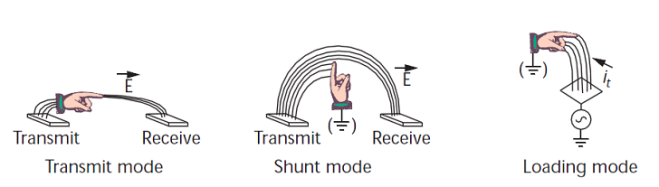
\includegraphics[width=0.6\textwidth]{images/cap_sensing_modes.png} 
\caption{Three measurement modes for capacitive proximity sensing \cite{Smith1996a}}
\label{fig:cap_sensing_modes}
\end{figure}
A classic work in the field of capacitive proximity sensing that will be referenced occasionally in this work is “Electric Field Imaging” by Joshua Smith \cite{Smith1999a}. One contribution was the introduction of different measurement modes in capacitive sensing, as shown in Figure \ref{fig:cap_sensing_modes}. 
Transmit mode is using a transmitting electrode that is coupled to a conductive object; in case of interaction applications typically the human body. The properties of an electric field generated with respect to a receiving electrode will therefore be dependent on the distance of this body, thus extending the achievable range.
Shunt mode similarly uses both a receiving and transmitting electrode generating a static field. However, there is no body coupled and any conductive object will ground the field, thus reducing the energy stored, which is measured. This setup is able to work with various transmitters on a single receiver, enabling a higher amount of virtual sensors using limited hardware. The third measurement mode is called loading mode. An oscillating field is induced on a single electrode measuring the capacitance relative to the environment. Any approaching grounded object results in an increased capacitance that is measured periodically.
\subsection{Materials and geometry}
Two major factors that have to be considered when designing an application based on capacitive sensors are the materials and geometry of the electrodes performing the measurements. The material of the electrode should be picked according to the desired application, i.e. if the interaction device has a flexible surface, conductive thread could be used, if it is solid and opaque, the application of solid metal electrodes is viable. Additionally there are other options for transparent materials. While we traditionally associate solid metals to antennas and electrodes this view can no longer be upheld. Transparent conductive layers have been in use for decades now, e.g. in car windows or solar technology. They typically rely on metal oxide layers, polymer layers or in recent years carbon nanotubes \cite{Moon2005}. The most common technology for usage in displays is projected capacitive touch that uses a multi-layer design of insulated ITO electrodes that are able to detect the movement of several objects close to the surface \cite{Barrett2010}. However, they are typically tuned to allow operation within a small distance of \(1cm\) or less. However, they are typically tuned to allow operation within a small distance of \(1cm\) or less. One recent work was evaluating different types of electrode materials in terms of their spatial resolution at different distances between object and electrode \cite{grosse2013opencapsense}, focusing on larger distance proximity measurements. They benchmarked both ITO and PEDOT:PSS. The first is a thin layer of indium-titanium-oxide, a highly conductive metal layer that possesses good optical properties. PEDOT:PSS is a conductive polymer that has a lower conductivity and slightly less appealing optical properties. In conclusion they evaluated that while copper has still the best properties, at least ITO can be considered a suitable alternative in applications that require optical clarity, as shown in the achievable spatial resolution given in Figure \ref{fig:cap_spatial_resolution}. 
\begin{figure} [h]
\centering
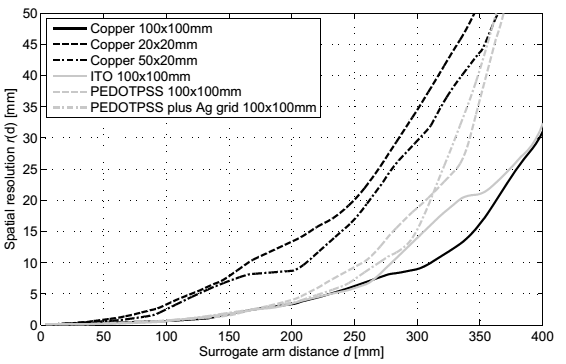
\includegraphics[width=0.6\textwidth]{images/cap_spatial_resolution.png} 
\caption{Spatial resolution of different materials at various distances \cite{grosse2013opencapsense}}
\label{fig:cap_spatial_resolution}
\end{figure}
The most common technology for usage in displays is projected capacitive touch that uses a multi-layer design of insulated ITO electrodes that are able to detect the movement of several objects close to the surface \cite{Barrett2010}. However, they are typically tuned to allow operation within a small distance of 1cm or less. 
Another area that is strongly influenced by the intended application is the geometry, whereas the electrode is considered the part of the electronics directly attached to the measurement circuit. This may range from simple straight wires or plate electrodes to complex optimized multidimensional structures specifically designed for a single task. Even though it is aimed at touch or near-proximity sensing we will give a short overview of  multi-layer designs for touch screens that have been reviewed by Barrett and Omote \cite{BarrettScreen}. They are designed to measure mutual capacitance, i.e. the resulting capacitive properties between a sending and a receiving electrode that are intersecting. If a sensible excitation and measuring process is used, multiple nearby objects may be reliably detected. 
\begin{figure} [h]
\centering
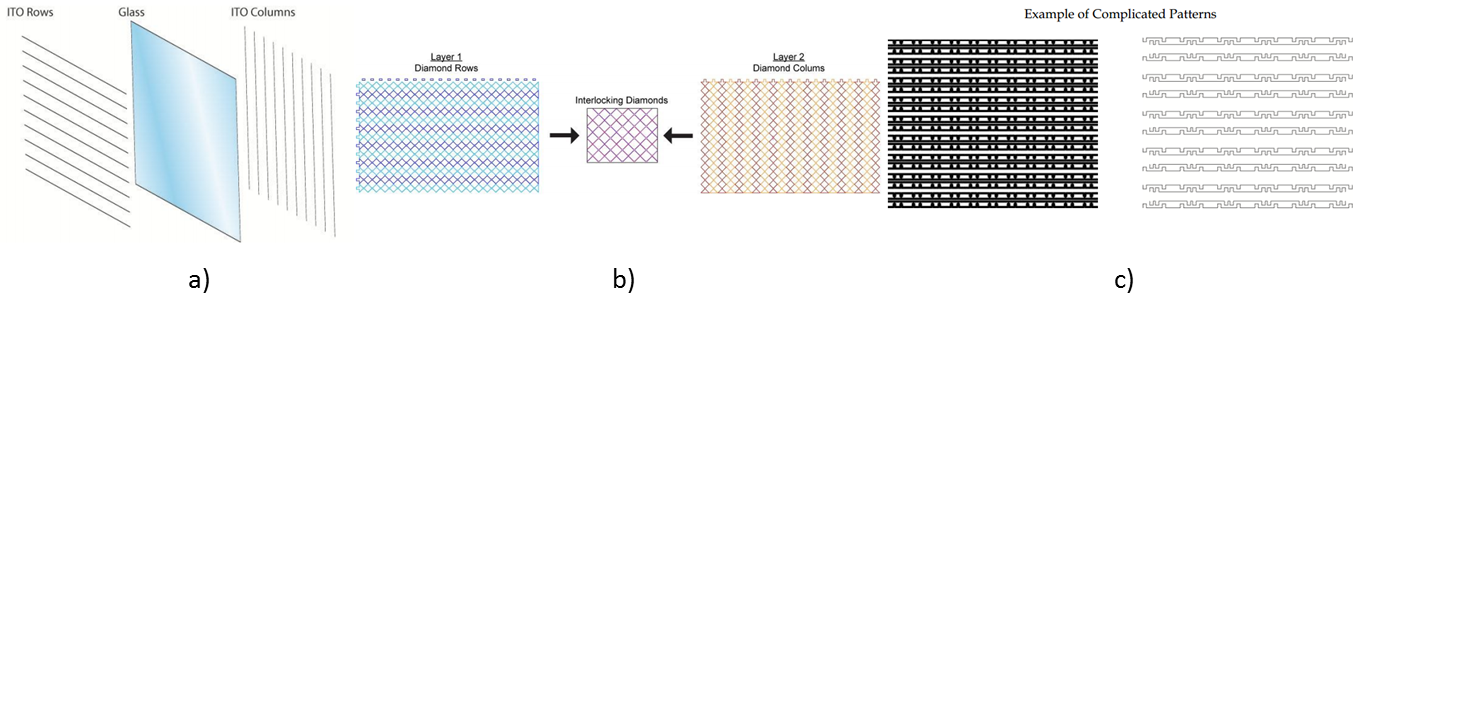
\includegraphics[width=0.8\textwidth]{images/ito_multilayer.png} 
\caption{Examples of multilayer layouts for touch screens - grid (a), interlocking diamonds (b) and  trademarked complex patterns (c) \cite{BarrettScreen}}
\label{fig:ito_multilayer}
\end{figure}
A simple example is two layers of perpendicular straight line electrodes - used by the first iPhone (Figure \ref{fig:ito_multilayer} - a). Another example uses an interlocking diamond shape \cite{Dietz2001a} to create a good spatial coverage (Figure \ref{fig:ito_multilayer} - b). Finally, there are numerous other complex patterns that are often trademarked by the companies that have developed the respective controller. One example is given in (Figure \ref{fig:ito_multilayer} - c). 

Capacitive proximity sensing applications are typically less concerned about intricate designs, but instead use varying electrode sizes and placement over a larger area. As previously mentioned the purpose of capacitive proximity sensing is the detection of objects and their properties. There are numerous factors that can influence the geometrical layout, but they can be abstracted into the following categories:
\begin{itemize}
\item	Number of objects
\item	Object size
\item	Desired spatial resolution
\end{itemize}
Going back to our example of touch screens, we have small objects, a higher number of those (usually up to 10) and require a high spatial resolution to select small items on the screen. The result is a fine multilayer grid, using mutual capacitance to simplify multi-object recognition, fine electrode spacing to achieve a high spatial resolution and thin or transparent electrodes to guarantee good optical properties. A similar rationale can be applied to other applications. If we take the smart couch by Große-Puppendahl et al. the aim is to detect the presence and posture of one or more persons on a couch \cite{Couch2011}. This necessitates detecting large body parts such as head, torso or limbs. There is no fine-grained spatial resolution required, allowing a reduction the number of sensors and it was assumed that a maximum of two persons are on the couch. Furthermore the electrodes are placed below the upholstery, thus requiring a reasonable detection distance. 
\begin{figure} [h]
\centering
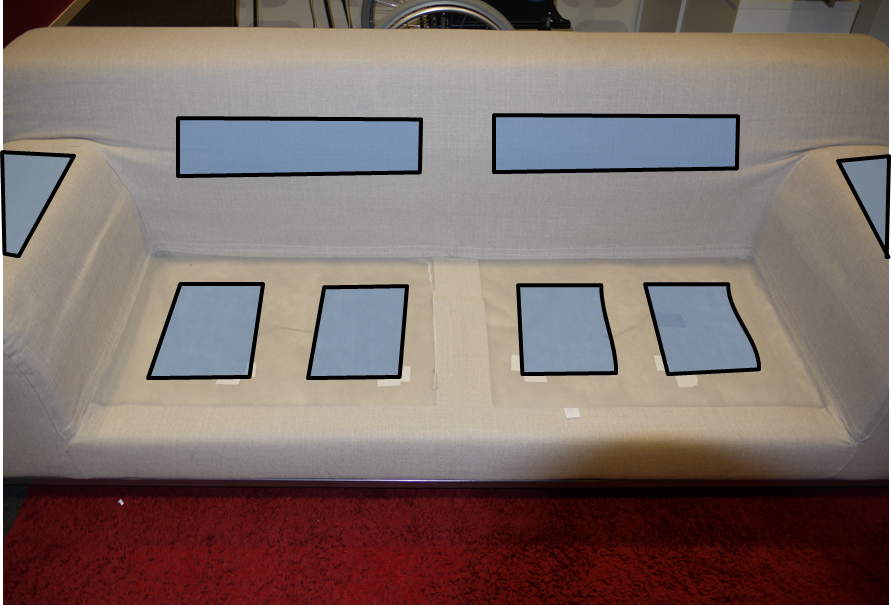
\includegraphics[width=0.7\textwidth]{images/couch_electrodes.png} 
\caption{Electrode placement below upholstery \cite{Couch2011}}
\label{fig:couch_electrodes}
\end{figure}
The resulting electrode placement can be seen in Figure \ref{fig:couch_electrodes}. The layout was designed under the additional constriction of using a single sensor kit, supporting up to eight electrodes. Regarding placement it is most important to distinguish two persons and different sitting positions, thus four electrodes are placed below the sitting area. In the back there are two electrodes spread over the entire width to determine the presence of the upper body close to the backrest. The electrodes in the armrests determine a head and are primarily suitable for detecting lying positions. In consequence this setup is suitable for detecting multiple sitting persons, infer information about their sitting position and recognize lying persons. Regarding those postures it showed good results in the prototype's evaluation \cite{Couch2011}.
 
A third and final example for the rationale of electrode placement is the TileTrack system by Valtonen et al, a capacitive person tracking system using floor tiles \cite{Valtonen2009a}. It is a transmit mode system that has the transmitting electrodes placed below the floor tiles and the receiving electrodes are placed in the walls of the area. The main goal of the system is the tracking of persons on the surface. Thus the floor area should be mostly covered by electrodes to establish a good transmission link to the bodies. The receiving electrodes should be able to pick up all signals generated by the body. Valtonen et al. picked wire or plate electrodes that went from floor level to a height of 190cm that covers most typical body sizes. While the system has some shortcomings with regard to applicability in larger rooms, the design rationale is appropriate for narrow rooms or when only movement close to walls has to be detected and had a reasonable precision in their evaluation.
Looking at the above examples it becomes apparent that the proper selection of materials and geometry is highly depending of the desired application. In consequence it is difficult to give generic guidelines independent of the application. After reviewing the different application domains in the next section we will revisit this topic in section 5.4.

\subsection{Data processing}
\begin{figure}[h]
\centering
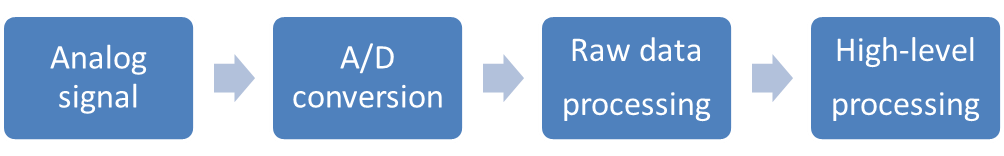
\includegraphics[width=0.4\textwidth]{images/proc_pipe}
\caption{Abstracted sensor data processing pipeline}
\label{fig:rel_proc_pipe}
\end{figure} 
%Figure 10 Abstracted sensor data processing pipeline
In order to acquire usable data from any digital sensor an analog signal has to be acquired and processed. A simplified typical processing pipeline for this is shown in Figure \ref{fig:rel_proc_pipe}. This basic structure is also applicable to the processing of capacitive proximity sensor data. The analog signal is the capacitance of an electric circuit that can be digitized using different methods, e.g. by using the quantized discharge time of the circuit. In the following section some typical steps of raw data processing and high-level processing for capacitive proximity sensors are presented and discussed. 
\subsubsection{Raw data processing}
Raw data processing of capacitive proximity sensor data is primarily intended to compensate for sensor noise and environmental influences. Noise is an inherent property of any measurement system and describes random unwanted data that is added to a signal. Environmental parameters can have strong influence on the signal of a capacitive sensor system. These effecting factors include temperature, humidity, composition of the air, or grounded objects in close proximity. There are numerous additional preprocessing steps that can be taken, such as different multiplexing methods that may be required in some hardware settings, or signal quantization that reduces the outgoing data to a distinct set of values in order to simplify post processing of different applications. These will not be further discussed in the scope of this work.
\paragraph{Noise Reduction}
In order to deal with noise, some sort of filtering is typically applied. Filtering describes a set of methods that attenuate the parts of a signal that are relevant in a given application. In capacitive proximity sensing we are dealing mostly with high-frequency noise that is added to the signal. Therefore, low-pass filtering can be used to deal with this influence. The most typical examples are average filters that take various samples and calculate an average value, and median filters that are sorting a set of samples and select the median element. Each of those filters has a plethora of potential adaptations that are not too specific to discuss in this limited space. Some adaptations are discussed in the specific prototype sections.
\begin{table}[htbp]
  \centering
  \caption{Baseline calibrations terms and methods}
    \begin{tabular}{lp{6cm}p{5cm}}
    \toprule
    \textbf{Name} & \textbf{Description} & \textbf{Application} \\
    \midrule
    \textbf{Initial calibration} & First set-up of baseline at system start, e.g. by taking the average over various samples & Required for any application \\
    \textbf{Static baseline} & Baseline that does not change at run-time & For static environments \\
    \textbf{Dynamic baseline} & Baseline that changes over time & For non-static environments \\
    \textbf{Drift } & Change of system response to environmental factors at run-time & - \\
    \textbf{Drift compensation} & Methods to account for occurring drift, by changing the baseline value & Non-static applications \\
    \textbf{Recalibration} & Change of the baseline value at a specific point in time given a set of rules & Non-static applications \\
    \bottomrule
    \end{tabular}%
  \label{tab:rel_baseline}%
\end{table}%


%Table 1 Baseline calibrations terms and methods
%Name	Description	Application
%Initial calibration	First set-up of baseline at system start, e.g. by taking the average over various samples	Required for any application 
%Static baseline	Baseline that does not change at run-time	For static environments
%Dynamic baseline	Baseline that changes over time	For non-static environments
%Drift 	Change of system response to environmental factors at run-time	-
%Drift compensation	Methods to account for occurring drift, by changing the baseline value	Non-static applications
%Recalibration	Change of the baseline value at a specific point in time given a set of rules	Non-static applications

\paragraph{Baseline Calibration}
A very important aspect of capacitive raw data processing is signal calibration. The generated electric field is subject to changes over time, if either intrinsic parameters change or the environment is modified. Some specific examples include the electronic components heating up, the environmental temperature changing, or objects being moved in and out of detection range. Therefore it is essential to have a well-calibrated and adaptive baseline; that is the sensor signal generated in the environment without the presence of any object that we want to detect. Again, there are numerous methods to adapt and configure the baseline. We have collected a few common terms and methods and give some pointers regarding their application. The results are shown in Table \ref{tab:rel_baseline}. 
\begin{figure}[h]
\centering
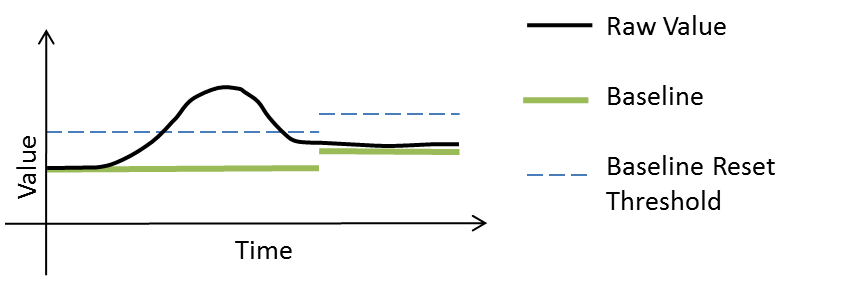
\includegraphics[width=0.5\textwidth]{images/baseline_reset}
\caption{Example of baseline reset using a threshold rule}
\label{fig:rel_base_reset}
\end{figure} 
%Figure 11 Example of baseline reset using a threshold rule
If a dynamic baseline is used, a set of rules will have to be defined that determines at which points in time the baseline has to be recalibrated, what specific methods should be used and the set of parameters that control the methods. One simple example is to define a threshold level that triggers a baseline calibration, as shown in Figure \ref{fig:rel_base_reset}. The raw signal is above the threshold, indicating the presence of a detectable object. Afterwards, it falls back down below the threshold, yet stays for a certain time above the baseline. This triggers a reset of the baseline after a certain amount of time.
\subsubsection{High-level processing}
High-level processing assumes that we already have calibrated (and possibly normalized) sensor values that are used in further steps. The goal of any capacitive sensing application is the acquisition of information about a detectable object, e.g. its current position, the material used or the shape. In order to get this information we need to use knowledge about the object and intrinsic properties of the sensor system. In this section we will discuss methods to combine data from various sensors using the system properties, how to track the position of an object using different methods and how to recognize specific features. An overview of the methods in abridged form is given in Table \ref{tab:rel_highlevel}. 
\begin{table}[htbp]
  \centering
  \caption{Overview of high-level processing methods for capacitive proximity sensors}
    \begin{tabular}{lp{5cm}}
    \toprule
    \textbf{Name} & \textbf{Description} \\
    \midrule
    \textbf{Sensor data fusion} & Combining sensor data into a shared representational format \\
    \textbf{Uniform fusion} & Sensor data fusion that combines all data into a single common format \\
    \textbf{Heterogeneous fusion} & Sensor data fusion that combines groups of data to serve multiple purposes \\
    \textbf{Object tracking } & Continuous identification of an object within the systems range \\
    \textbf{Single object tracking} & Methods to realize object tracking for a single detectable object \\
    \textbf{Multiple object tracking} & Methods to realize object tracking for multiple objects \\
    \textbf{Feature recognition} & Identifying certain parameters of an object within the system range \\
    \bottomrule
    \end{tabular}%
  \label{tab:rel_highlevel}
\end{table}%

%Table 2 Overview of high-level processing methods for capacitive proximity sensors
%Name	Description
%Sensor data fusion	Combining sensor data into a shared representational format
%Uniform fusion	Sensor data fusion that combines all data into a single common format
%Heterogeneous fusion	Sensor data fusion that combines groups of data to serve multiple purposes
%Object tracking 	Continuous identification of an object within the systems range 
%Single object tracking	Methods to realize object tracking for a single detectable object
%Multiple object tracking	Methods to realize object tracking for multiple objects
%Feature recognition	Identifying certain parameters of an object within the system range

\paragraph{Sensor data fusion}
Sensor data fusion in its most general terms describes “the theory, techniques and tools which are used for combining sensor data, or data derived from sensory data, into a common representational format” \cite{mitchell2007introduction}. Using the combined information from various capacitive proximity sensors we are able to generate high-level information that exceeds the capabilities of a single sensor. We can distinguish uniform fusion that uses the information from all involved sensors in one common way or heterogeneous fusion that combines groups of involved sensors that serve multiple purposes, yet are attached to a single system. A simple example for the latter would be a single large electrode sensor that detects the presence of a hand from a farther distance and then a combination of various small electrodes that track single fingers. 
Sensor data fusion often requires taking into account some additional information we possess about the system. A classic example is the precision or bias of the sensor. Various methods, e.g. the class of Kalman filters, use weighted information from several sensor sources \cite{welch1995introduction}. If we know how that a certain sensor is only half as precise as another one working in collaborating, the weighting factors can be adapted accordingly. 

One of the most important additional information we use when fusing data of capacitive proximity sensors, is the geometric layout of the system. This describes position and size of all electrodes that are integrated. Using this information is crucial when trying to localize an object. A simple example would be applying a weighted average algorithm on a set of sensors. In order to determine object location relative to the plane a weighted average algorithm is used. The linear object location $\overline{x}$ is calculated using the sums over sensor positions $x_i$ and sensor values $v_i$ as weight:
\[\overline{x}=\frac{\sum^n_{i=1}{v_i x_i}}{\sum^n_{i=1}{v_i}}\]

Using similar methods we are able to determine the location of multiple objects or additional dimensions of the position.
However, it is possible to use other information in the fusion process as well. The electrode material may result in a different response and thus should be treated differently in a fused data representation and can be weighted. Another example is the shape of the electrode that may result in different responses. How to apply sensor data fusion is strongly depending on the application and the desired common representation that is most suitable for subsequent calculations.

\paragraph{Object tracking}
In the previous section about sensor data fusion we have shortly discussed a method to determine the linear position of a single object using a linear array of capacitive proximity sensor. This is a basic example of a group of methods associated to object tracking. In computer vision applications they can be defined as “the problem of estimating a trajectory of an object in an image plane as it moves around a scene” \cite{yilmaz2006object}. The analogy to capacitive applications is viable if we consider a 3D scene and a distinct interaction space instead of a scene. 
Capacitive proximity sensors allow the detection of conductive objects within their range. However, as this presence is determined indirectly using the influence on an electric field it is not possible to get a direct association between the actual distance between sensor and object and the resulting sensor value. The created electric field is only analytically descriptive for very specific, theoretic classes of objects \cite{Baxter1996}. Nonetheless, we are able to get a relative distance measurement. If we combine this proximity value using geometric information about the electrode location we can infer the relative position of an object in the sensing area. The weighted average method presented in the previous section is one option for relative positioning. Another method is trilateration, similar to many radio-based localization applications, that uses the known location of three or more points and the known distance to the position to be determined. In case of capacitive proximity sensing this position is determined relative to the electrodes as there is no absolute distance measurement. 
A more complex example for direct calculation was presented by Smith, who formulated the issue of detecting multiple objects as a forward problem and used numerical methods to estimate the position and orientation of two hands \cite{Smith1999a}.
\begin{figure}[h]
\centering
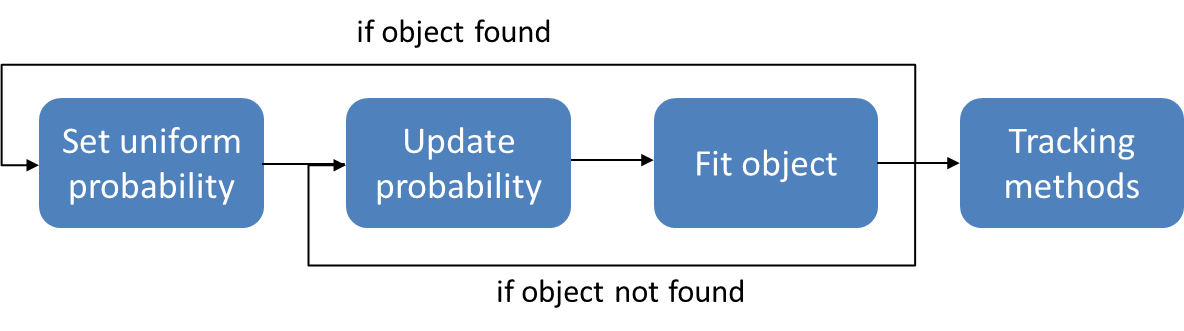
\includegraphics[width=0.5\textwidth]{images/prob_methods}
\caption{Generic pipeline of probability based methods of capacitive proximity sensing}
\label{fig:rel_prob_method}
\end{figure}
%Figure 12 Generic pipeline of probability based methods of capacitive proximity sensing
A second class of methods to track objects is not relying on direct geometrical calculations but instead formulates a numerical solution to a probability distribution. The initial assumption is that the probability of an object to be at a certain point in the detection area is uniform. The methods then follow a few basic steps, as shown in Figure \ref{fig:rel_prob_method}. At first the probability is updated based on the current sensor readings and a priori knowledge that we have about the system. Afterwards we try to fit the objects into the resulting probabilities. This step may or may not work, meaning that it may result in no object found. In the latter case the process will have to start at the beginning. If an object is found the probability update may use the current object location in the update algorithm, thus starting with a non-uniform probability distribution.
One example for probability-based object recognition using capacitive proximity sensors was presented by Grosse-Puppendahl et al. \cite{grosse2013swiss}. Using a model suggested by Smith the basic idea is using the assumption that an object may be present anywhere, remove regions where no objects can be present and then fit an object into the remaining space. This method additionally uses particle filters to track object locations over time. This also allows tracking multiple objects. 
Throughout the years various methods have been suggested for supporting multi-object tracking using capacitive sensors. Touch screens often use inversion of the sender signal to reliably detect the positions of multiple points; however, this method can’t be used in proximity applications \cite{wilson2007}. Some of the previously presented methods support the tracking of two or more objects. There are still various limitations, particularly if not only the object location but also various other features such as rotation should be tracked. This is still an area of ongoing research, leading to the next area of high-level processing - feature recognition.
\begin{table}[htbp]
  \centering
  \caption{Feature recognition methods}
    \begin{tabular}{lp{7cm}}
    \toprule
    \textbf{Name} & \textbf{Description} \\
    \midrule
    \textbf{Data-driven  methods} & Directly associate input data to output features using various methods, e.g. machine learning and training data \\
    \textbf{Model-driven methods} & Input data is manipulating a pre-defined model of the system that is latter mapped to the output \\
    \textbf{Neural networks} & Computational models using a network of neuron-like objects that are often used in machine learning \\
    \textbf{Pattern recognition} & Methods that look for certain patterns in a set of input data \\
    \textbf{Semantic mapping} & Methods to realize object tracking for a single detectable object \\
    \bottomrule
    \end{tabular}%
  \label{tab:rel_feature}%
\end{table}%

%Table 3 Feature recognition methods
%Name	Description
%Data-driven  methods	Directly associate input data to output features using various methods, e.g. machine learning and training data
%Model-driven methods	Input data is manipulating a pre-defined model of the system that is latter mapped to the output
%Neural networks	Computational models using a network of neuron-like objects that are often used in machine learning
%Pattern recognition	Methods that look for certain patterns in a set of input data
%Semantic mapping	Methods to realize object tracking for a single detectable object

\paragraph{Feature recognition}
Feature recognition is primarily used as a term in image processing, traditionally in computer-aided design applications to recognize specific geometric properties of an object but also picture analysis, e.g. in facial recognition \cite{han2000manufacturing}\cite{belhumeur1997eigenfaces}. 
In the domain of capacitive proximity sensing, feature recognition can be defined as the acquisition of non-location information from any detectable object. An important feature in industrial applications is the material of an object \cite{Baxter1996}. With regards to recognizing additional features a system was presented by Wimmer et al. - Thracker \cite{Wimmer2006}, a prototype augmenting a regular monitor with capacitive proximity sensors. In addition to recognizing hand position the system is able to detect grasp gestures, which can be used to select items on the screen and perform pick and drop operations. Capacitive sensors can also be used to distinguish between persons and a children’s seat on the passenger side of a car \cite{george2009seat}. 
The methods to recognize the features can be divers, ranging from typical machine learning algorithms, to model-based approaches. An incomplete list is given in Table \ref{tab:rel_feature}. In order to keep this work contained we refrain from a deeper discussion at this point.


\section{Capacitive proximity sensing applications}
\label{ch:rel_capapps}
\begin{minipage}{\linewidth}
\centering
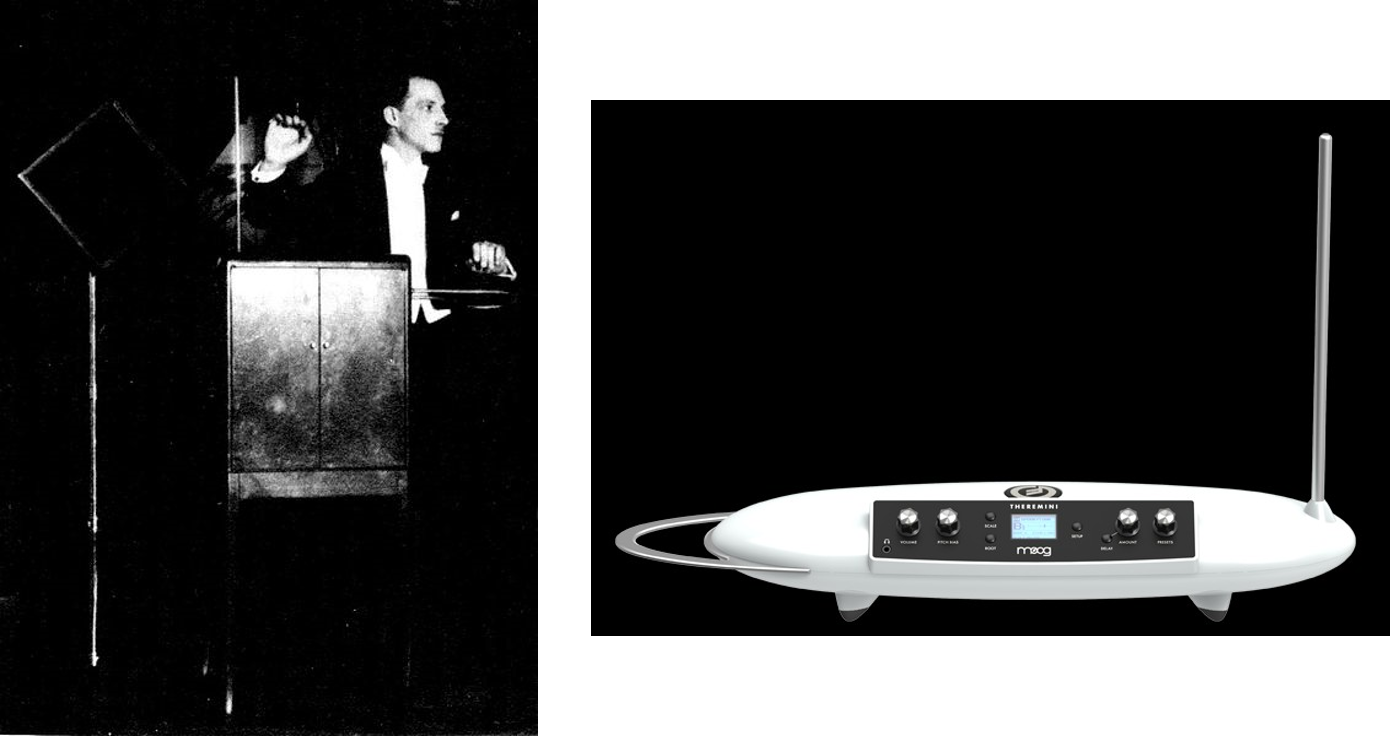
\includegraphics[width=0.9\textwidth]{images/theremins}
\captionof{figure}{\emph{Left:} Leon Theremin playing his epnoymous electronic musical instrument \cite{Glinsky2000}. \emph{Right:} The Theremini by Moog Music Inc., released in 2014 \cite{moog2014}}
\label{fig:theremins}
\end{minipage}
In the last decades of the 19th and the beginning of the 20th century a considerable number of inventors and scientists performed research on the application of electric systems, sparking innovations such as electric lighting, electric motors, telegraphy, and radio communication. Lev Sergeyevich Termen or Léon Theremin in the American naming was a Russian inventor most famous for designing the eponymous theremin. This early electronic musical instrument could be played without touch. One hand is controlling the pitch and the other the volume by changing the distance to an antenna. Initially designed as a motion detector, this device is transferring the influence of the human body on an oscillating electric field to an audible sound \cite{Glinsky2000}. Léon Theremin can be seen playing the instrument in Figure \ref{fig:theremins} on the left. This instrument is still in production to this day, with the electronic music instrument company Moog releasing a new variety that simplifies the sound production by fitting the distance to a sound on a specific musical scale \cite{moog2014}. The instrument is shown in Figure \ref{fig:theremins} on the right.

Electric field imaging was a research focus at the MIT in the 1990s. A research group in the Media Lab division including Joseph A. Paradiso, Thomas G. Zimmerman, Joshua R. Smith designed various sensing devices and evaluated various applications in in the domains of human computer interaction, smart appliances and reactive systems. They drew inspiration from biological precedents - various species of fish, such as Gymnotoidei can sense their surroundings using electric fields \cite{smith1999thesis}. The changing currents created by objects with a different dielectric constant from water can be registered and thus used to avoid obstacles, even if no light source is available. Accordingly, the group named some of their prototypes after this biological precedent, including the LazyFish and School of Fish \cite{smith1999thesis}. The research group created various different applications in the domains of human computer interaction, smart appliances and reactive systems.

\begin{minipage}{\linewidth}
\centering
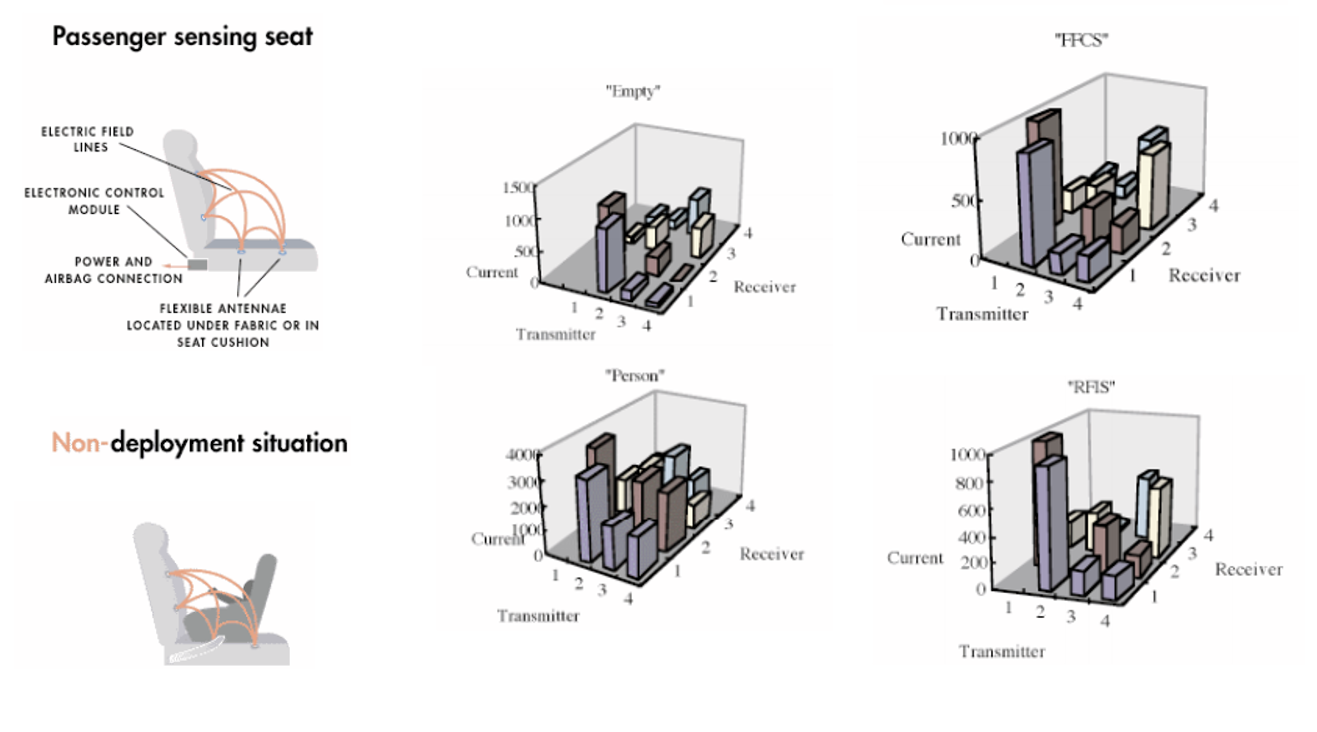
\includegraphics[width=0.9\textwidth]{images/nec_passenger_seat}
\captionof{figure}{\emph{Left:} Concept view of passenger seat set to deploy or not deploy airbag. \emph{Center:} Sensor readings for empty seat and adult person. \emph{Right:} Sensor readings for front-facing child seat (FFCS) and rear-facing child seat (RFCS). \cite{smith1999thesis}}
\label{fig:nec_passenger_seat}
\end{minipage}

In collaboration with NEC a smart passenger seat was created that incorporated capacitive sensors operating in shunt mode to detect if an infant seat is currently present on the passenger seat of car \cite{grosse2012enhancing}. The underlying challenge is that an airbag deployment should be prevented in such cases to prevent potential injuries to the infant. The seat is able to distinguish four different states, “No passenger”, “adult passenger”, “front-facing infant seat” and “rear-facing infant seat”. It uses four sending and four receiving electrodes and classifies the situation according to the current readings - the concept and readings of the sensors in the different situations are shown in Figure \ref{fig:nec_passenger_seat}.

\begin{minipage}{\linewidth}
\centering
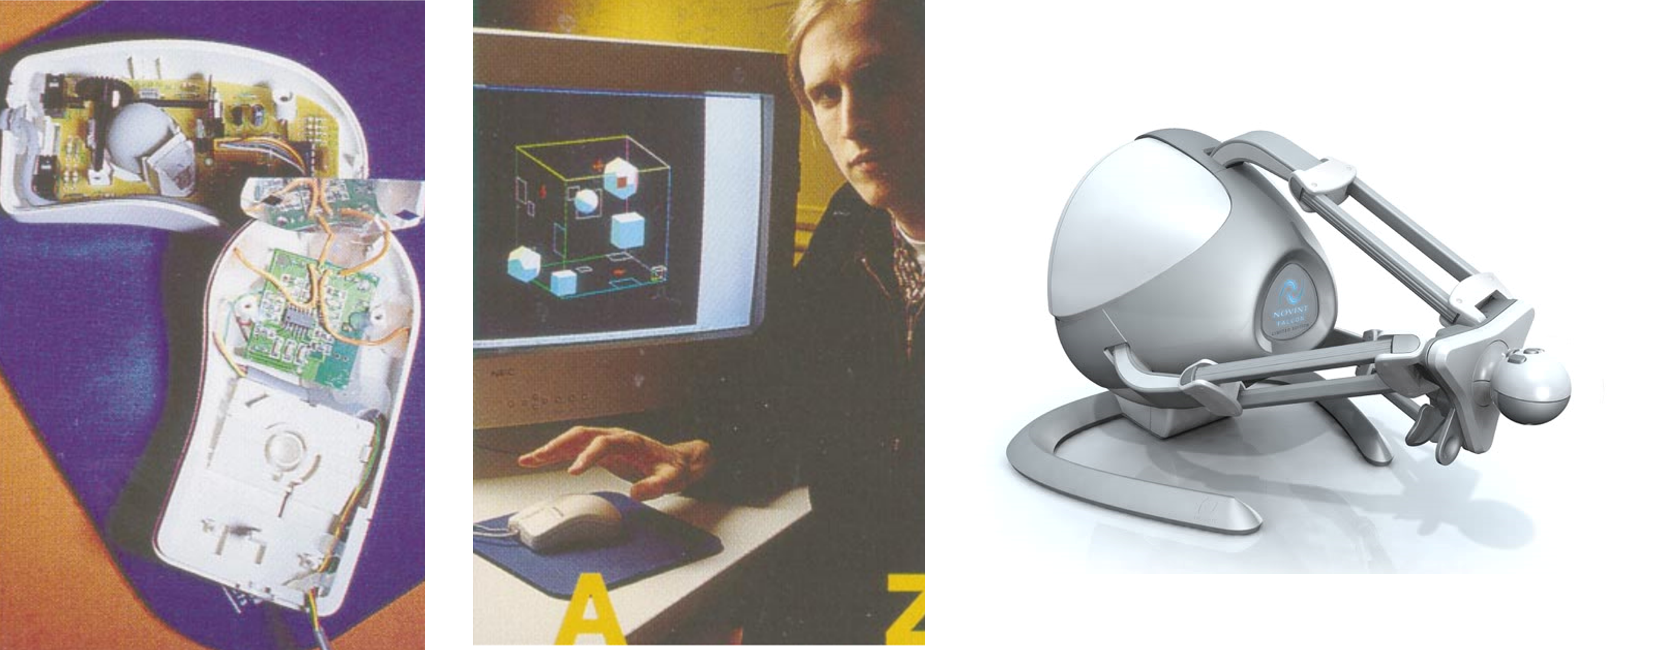
\includegraphics[width=0.9\textwidth]{images/lazmouse}
\captionof{figure}{\emph{Left:} LaZmouse innards \emph{Center:} Joshua R. Smith using LaZmouse \cite{smith1999thesis} \emph{Right:} Novint Falcon 3D input device \cite{novint2014}}
\label{fig:lazmouse}
\end{minipage}

Another prototype is the LaZmouse that extends a regular mouse with shunt mode capacitive sensors, having one transmitting and two receiving electrodes, to measure the proximity between the heel of the hand from the mouse surface, thus allowing the fingers to remain in the common position and the mouse to be moved around \cite{smith1999thesis}. Effectively this creates an input device with three degrees-of-freedom, enabling to perform interactions with a mouse that would usually require a more specialized 3D input device, such as the Novint Falcon that tracks the movement of the moved interaction sphere in three dimensions \cite{novint2014}. Figure \ref{fig:lazmouse} shows on the left, the electronics inside the mouse, the inventor using the device and a graphical representation, and on the right the Novint Falcon.

In another work Paradiso et al. presented numerous applications for capacitive proximity sensors, including smart furniture devices \cite{ Zimmerman1995}. They propose a smart table, comprised of a single transmitter electrode and two receivers that is able to track the position of a hand in two dimensions, a chosen dimension on the table and height. It may be used as gesture input device or to augment video desk applications. They also installed the system in a room, whereas the floor is a single electrode and there are four receivers located on the walls. This allows to infer the location of a person, based on relative signal strength. An additional system in this work is the smart chair, using a single transmitter in the seat and four receivers in the armrests and headrest. It allows to navigate through various audio channels based on head and arm movements \cite{ schmandt1995audiostreamer}.

\begin{minipage}{\linewidth}
\centering
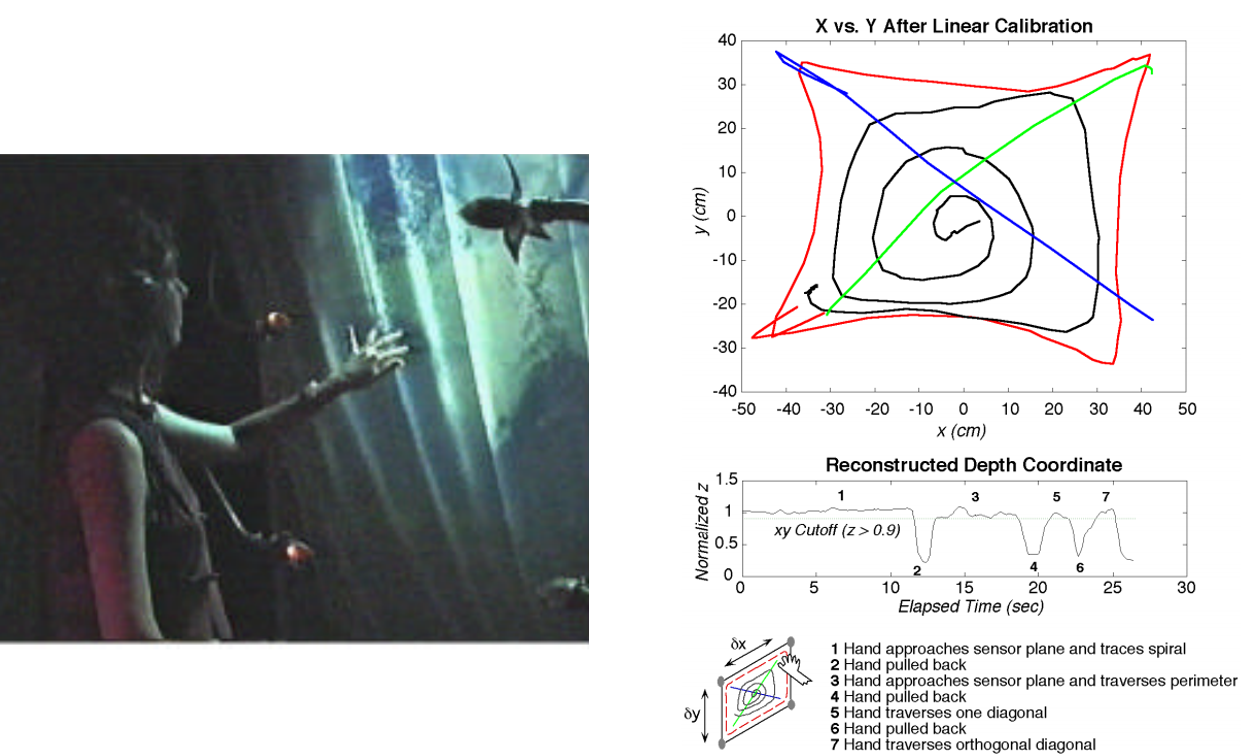
\includegraphics[width=0.8\textwidth]{images/related_gesture_wall}
\captionof{figure}{\emph{Left:} Person interacting with the gesture wall  \emph{Right:} Air drawing results, depth estimation results and associated movements on bottom. \cite{smith1998electric}}
\label{fig:related_gesture_wall}
\end{minipage}

A final prototype of this group I would like to present is the Gesture Wall, a large interactive multimedia wall, designed for public appearances \cite{smith1998electric}. A plate on the floor in front of the screen is acting as transmitter and four receiving electrodes that protruded from the edges of the projection area, as shown in Figure \ref{fig:related_gesture_wall}. It supports interactive experiences, such as drawing in the air, controlling different audio streams and an interactive video clip.

\begin{minipage}{\linewidth}
\centering
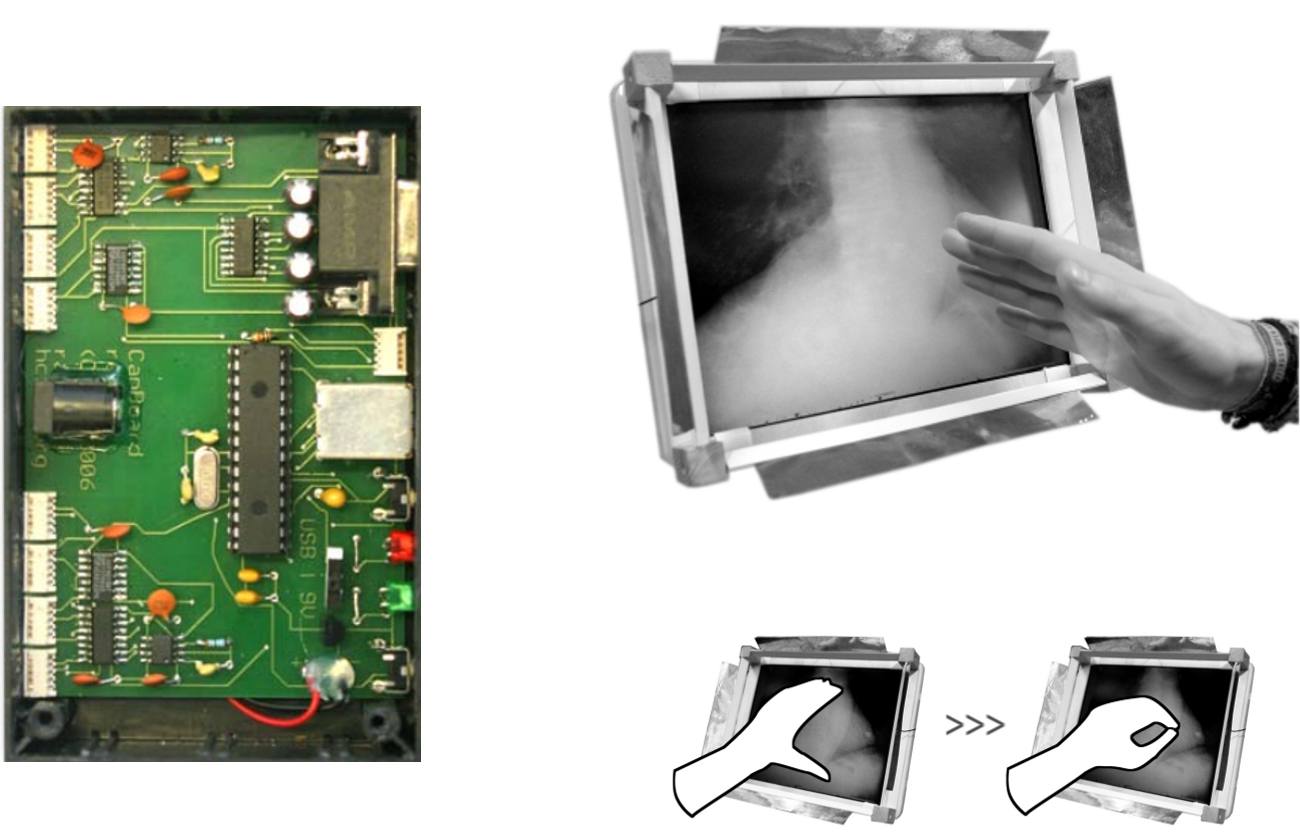
\includegraphics[width=0.9\textwidth]{images/related_ctk_thracker}
\captionof{figure}{\emph{Left:} Prototype of CapToolKit  \cite{Wimmer2007a} \emph{Right:} Thracker prototype and visualized grasping gestures. \cite{Wimmer2006}}
\label{fig:related_ctk_thracker}
\end{minipage}

Another group that was active in capacitive proximity sensing was located at the University of Munich. Raphael Wimmer and colleagues revisited capacitive sensors in the scope of human-computer interaction. They created CapToolKit, a capacitive sensing rapid prototyping toolkit that allows interfacing eight capacitive proximity sensors and enables a quick design and testing of new applications  \cite{Wimmer2007a}. They also created Thracker - a display augmented with four capacitive proximity sensors that allows to detect the position of the hand in front of the screen and supports performed pick-and-drop gestures \cite{Wimmer2006}. Both devices are shown in Figure\ref{fig:related_ctk_thracker}.

\begin{minipage}{\linewidth}
\centering
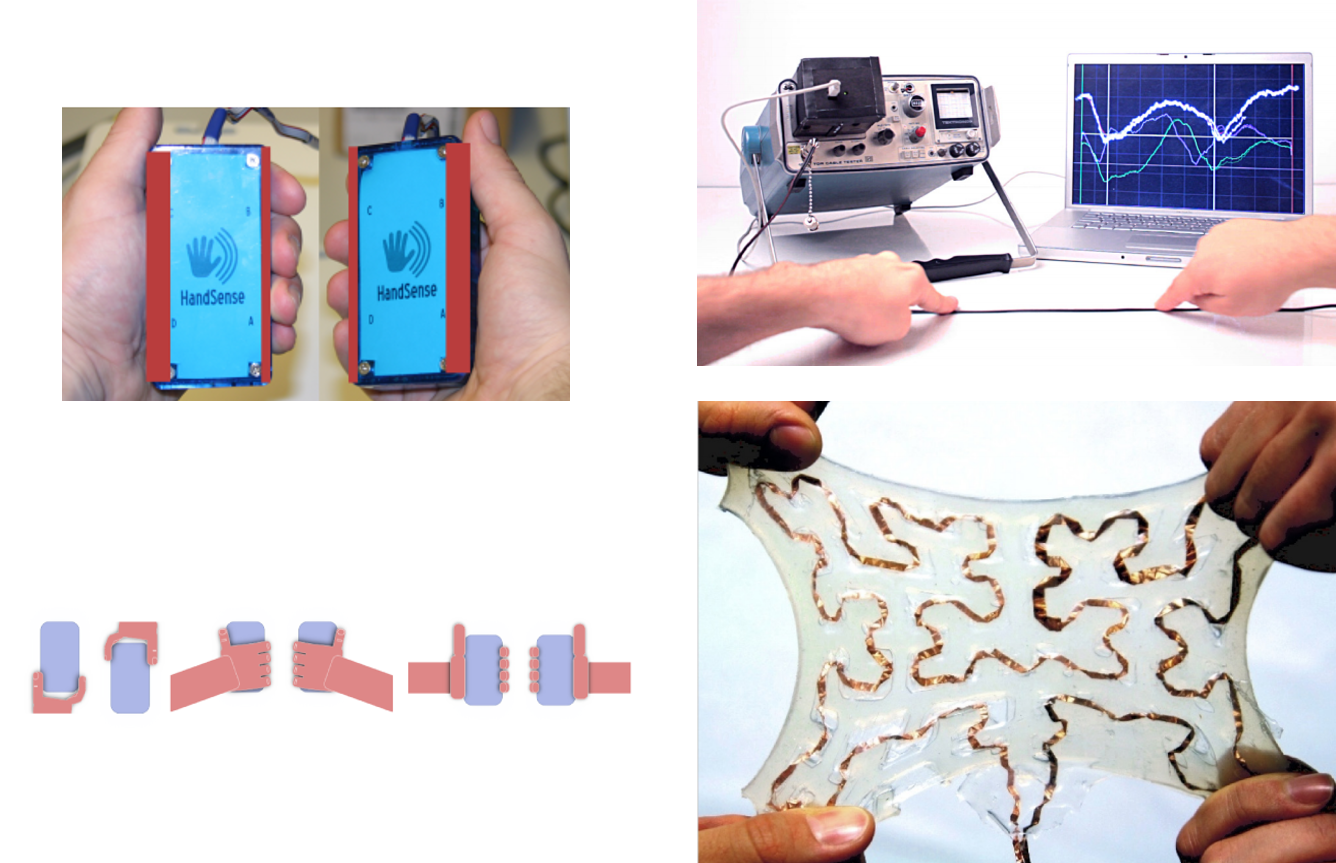
\includegraphics[width=0.8\textwidth]{images/related_handsense_tdr}
\captionof{figure}{\emph{Left:} Prototype of HandSense and supported grasping types \cite{wimmer2009handsense}. \emph{Right:} Setup of time domain reflectometry sensing and example of stretchable material \cite{wimmer2011modular}.}
\label{fig:related_handsense_tdr}
\end{minipage}

In other works they also presented capacitive sensing to allow discriminating the ways an interaction device is held, including distinguishing left and right hand or proximity to a body part \cite{ wimmer2009handsense}. This enables graphical interfaces to be adapted, based on user-handedness, grasping style and spatial cues that can be acquired from this device in collaboration with other sensors. Supported grasping styles and a prototype are shown in Figure \ref{fig:related_handsense_tdr}, on the left.

A final work of this group was concerned with exploring the potential of time domain reflectometry for human-computer interaction \cite{wimmer2011modular}. This technique is sending a short electrical pulse into an electric conductor and measures the time until the signal returns. Originally intended for finding defects in long cables, such as transatlantic phone lines, high-sampling rates enable to also detect the presence of grounding objects close to much shorter conductors. Wimmer and Baudisch use an image analysis on the screen of an older reflectometer to enable applications, such as location tracking, touch detection and stretchable materials. The setup and an example of stretchable materials are shown in Figure \ref{fig:related_handsense_tdr}, on the right.

\begin{minipage}{\linewidth}
\centering
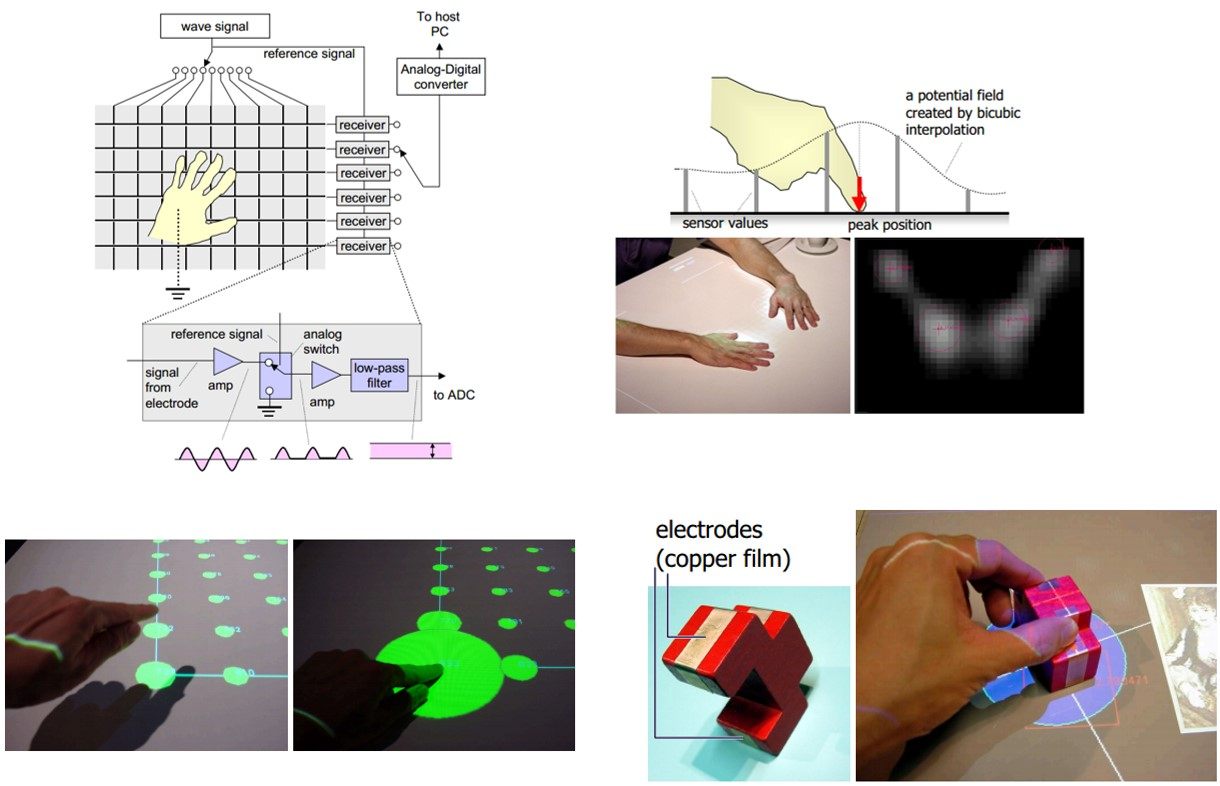
\includegraphics[width=0.8\textwidth]{images/capapp_smartskin}
\captionof{figure}{\emph{Top left:} Technical configuration of SmartSkin. \emph{Top Right:} Bicubic interpolation method to detect the peak of the potential field created by hand proximity. \emph{Bottom left:} Visualized sensor effect of hand hovering in 10 cm distance and touching the surface. \emph{Bottom right:} Capacitance tag having a specific conductive pattern that can be identified \cite{rekimoto2002smartskin}} 
\label{fig:capapp_smartskin}
\end{minipage}

Jun Rekimoto presented SmartSkin, an interactive table based on capacitive proximity sensing based on a number of sensors configured in shunt mode \cite{rekimoto2002smartskin}. They are able to detect hands and fingers at a distance of up to 10 cm, the sensor response being shown in Figure \ref{fig:capapp_smartskin} on the bottom left. He investigated two different prototypes based on this technology and developed an image-based method to detect the position of hand or fingers above the surface, as shown in Figure \ref{fig:capapp_smartskin} on the top right. Additionally, capacitive tags were introduced that enable tangible interaction by detecting the type of object the user is currently touching on top of the surface, analyzing their specific capacitance pattern, resulting from a difference in shape and layout of conductive material covering the object, shown in Figure \ref{fig:capapp_smartskin} on the bottom right.

\begin{minipage}{\linewidth}
\centering
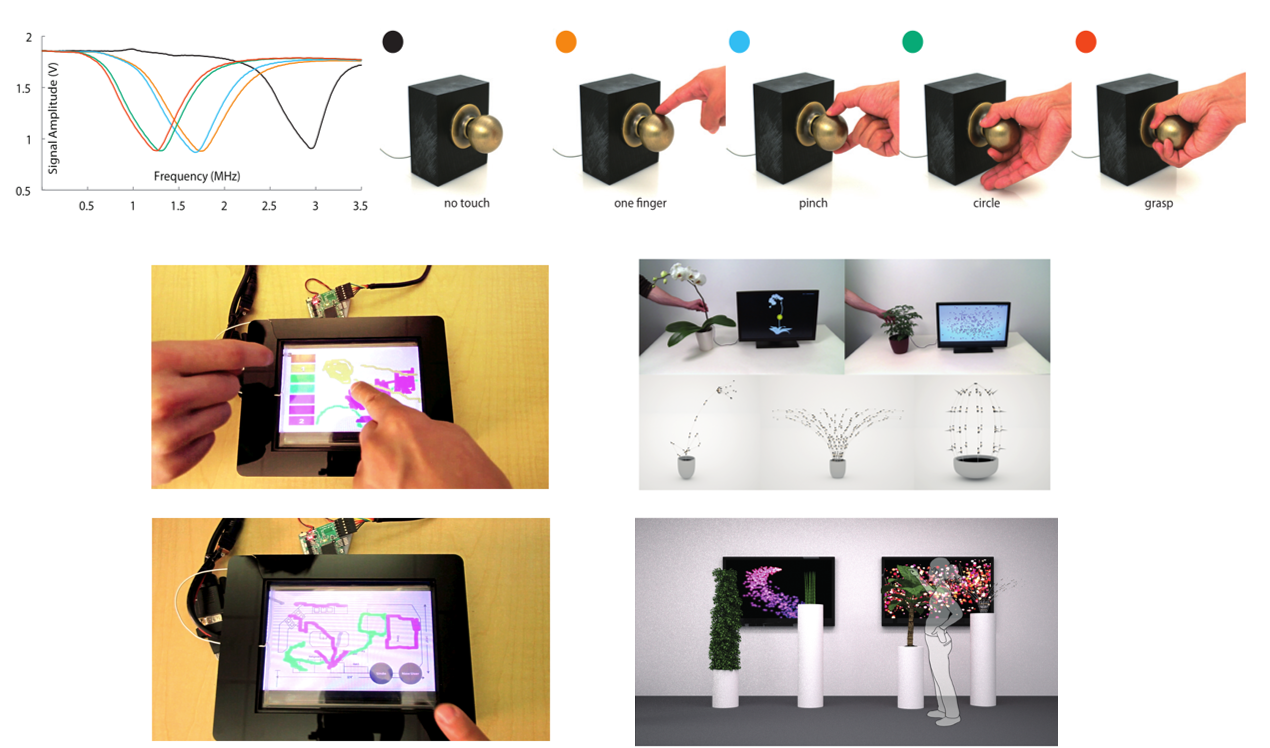
\includegraphics[width=0.8\textwidth]{images/rel_cap_disney}
\captionof{figure}{\emph{Top:} Capacitive profiles of different gestures on a door knob \cite{Sato2012}. \emph{Bottom Left:} User identification using capacitive fingerprinting \cite{harrison2012capacitive}. \emph{Bottom Right:} Botanicus Interacticus prototype and interaction concept \cite{poupyrev2012botanicus}} 
\label{fig:rel_cap_disney}
\end{minipage}

Another research group that has been recently active with capacitive sensing systems is centered around Ivan Poupyrev. They presented Touché, proposing a novel sensing technology called swept-frequency capacitive sensing \cite{Sato2012}. Instead of relying on a single excitation frequency like typical capacitive sensors this measurement system is sweeping a larger range of frequencies, thus allowing to get more data points from a single electrode. Many systems react differently to changing frequencies, including the human body and its complex structure of bone, muscle, fat and other tissues. The result is a capacitive profile comprised of values at different frequencies, as shown in Figure \ref{fig:rel_cap_disney} on the top. Using these profiles it is possible to distinguish numerous events based on the application, e.g. the different ways in which a mobile device can be held. Other applications proposed in this work were sensing of body postures on a table, on-body gestures using wrist-worn sensors, interaction with a body of water and grasping a door knob using different gestures. Building on this work Harrison et al. proposed a system using this technology to identify the users of a touch screen with a capacitive fingerprint \cite{harrison2012capacitive}. This allows to distinguish the touches of different users, thus enabling a variety of applications on collaboratively used touch screen devices, such as gaming and multiuser drawing tools, as shown in Figure \ref{fig:rel_cap_disney} on the bottom left. An interesting suggestion are personalized undo stacks that allow a more seamless collaboration. A final system is the Botanicus Interacticus, that uses the same technology to realize interactive installations using plants  \cite{poupyrev2012botanicus}. It is possible to distinguish the location a certain plant is touched and associate it to different input events. In this first system it was used in an interactive art installation, that is shown in Figure \ref{fig:rel_cap_disney} on the bottom right.

\begin{minipage}{\linewidth}
\centering
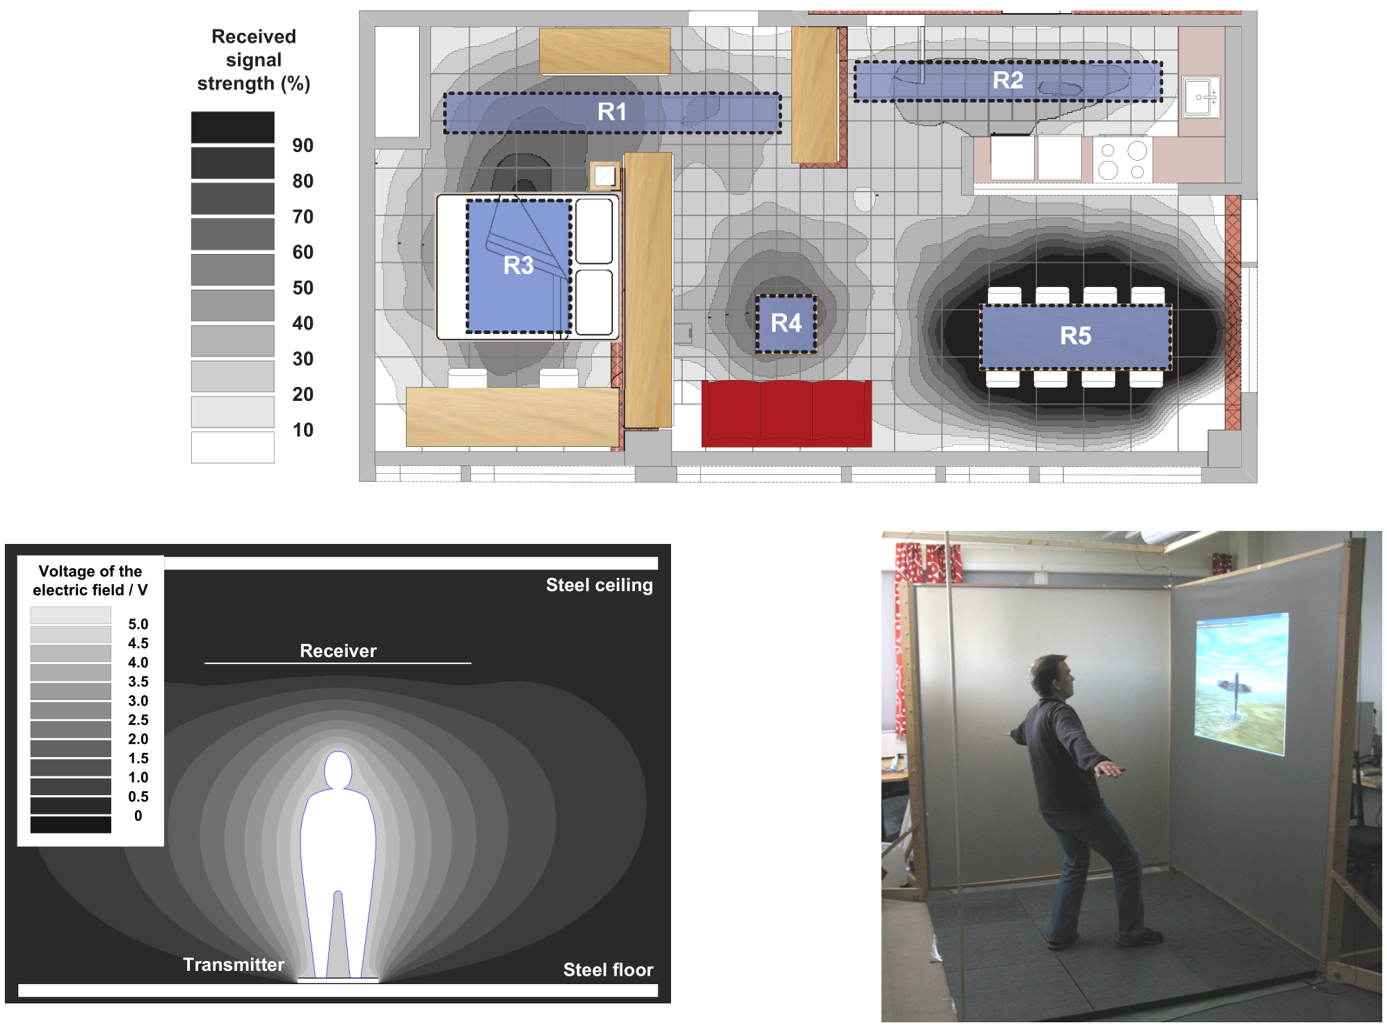
\includegraphics[width=0.8\textwidth]{images/rel_cap_tampere}
\captionof{figure}{\emph{Top:} Capacitive profiles of different gestures on a door knob \cite{Sato2012}. \emph{Bottom Left:} User identification using capacitive fingerprinting \cite{harrison2012capacitive}. \emph{Bottom Right:} Botanicus Interacticus prototype and interaction concept \cite{poupyrev2012botanicus}} 
\label{fig:rel_cap_tampere}
\end{minipage}

A final research group working with capacitive proximity sensing that I would like to present is located at the Tampere University of Technology. Valtonen et al. have been working on a capacitive proximity sensing system tracking the position of users in a room \cite{Valtonen2009a,valtonen2012capacitive}. A transmitting electrode is placed under the floor and several receiver electrodes are hidden in the walls or other objects of the room. The system therefor is using the presented transmit mode, coupling the users present in the environment to an electrode in the floor and measuring the effect on the receiver electrodes. A downside of this system is the required proximity to a wall electrode, making application in larger rooms impossible. Accordingly, an addition was presented that hides the receiving electrodes in different items of furniture to provide a more reliable localization in living environments \cite{valtonen2012capacitive}. The placement of the receiver electrodes (R) and the received signal strength in the environment are shown in Figure \ref{fig:rel_cap_tampere} on the top. An extension of this principle is using a similar electrode configuration to  determine height and posture of a person between a transmitter electrode on the bottom and a receiver electrode on the ceiling \cite{valtonen2011unobtrusive}. A simulation of the electric field voltages created in this setup is shown in Figure \ref{fig:rel_cap_tampere} on the bottom left. The taller a person, the higher the resulting signal. Accordingly, a sitting or lying person will have a much smaller effect and can be classified. A similar setup was also used to identify different gestures performed in an interaction area, as shown in Figure \ref{fig:rel_cap_tampere} on the bottom right \cite{valtonen2010human}. Using a single transmitter and four wire receivers in the corners it is possible to track different body postures and control some example applications.

\begin{minipage}{\linewidth}
\centering
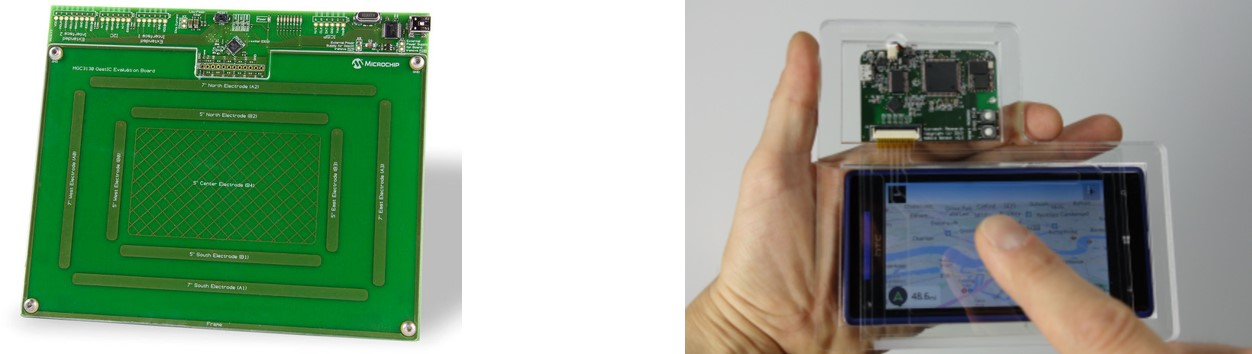
\includegraphics[width=0.8\textwidth]{images/cap_gestic}
\captionof{figure}{\emph{Left:} GestIC sabrewing prototyping board \cite{microchip2013}. \emph{Right:} Transparent interaction device based on GestIC \cite{le2014low}} 
\label{fig:cap_gestic}
\end{minipage}

Recently capacitive gesture interaction has also captured the interest of industry. GestIC by Microchip Technologies Inc. is a controller for electric near field 3D tracking based on capacitive proximity sensing \cite{microchip2013}. A prototyp1ing board is shown in Figure \ref{fig:cap_gestic} on the left. Using a set of several electrodes and on-board processing it is capable of tracking the 3D position of a hand and provides gesture recognition at a distance between 0 and 15 cm. It is based on shunt mode sensing and has a number of different available electrode configurations. This system was used in a recent publication by Le Goc et al. \cite{le2014low}. They used a transparent ITO electrode configuration mimicking the prototyping board configuration and presented a novel machine learning method, that improves the precision of the object localization. They presented a prototype system, augmenting a mobile device with 3D gesture interaction, as shown in Figure \ref{fig:cap_gestic} on the right.




\section{Sensor systems in smart environments}
\label{ch:rel_sensor_tech}
In the most general definition a sensor is a device that transforms a physical property into an observable signal. This definition includes traditional systems such as mercury-based thermometers or hair-based hygrometers. Yet nowadays we are usually considering digital sensors that transfer the measured property to a binary signal that can be further processed by computing devices. 
A common variety is the smart sensor that provides additional functionality beyond generating a correct sensing signal \cite{frank2013understanding}. The main goal is to simplify installation and maintenance of distributed sensing systems by having processing close to the measurement device. Early considerations in this domain were put to the standard family IEEE 1451 - IEEE Standard for a Smart Transducer Interface for Sensors and Actuators between 1997 and 2007 \cite{ieee1451}. An additional concept is the Virtual Sensor that includes digital signal processing and conditioning and therefor abstracts the processing steps from devices interfacing the sensor. 
The number of available sensors is very high, but it is possible to restrict them based on application domain. Lewis and Cook et al. \cite{lewis2004wireless,cook2007smart} have proposed a collection for smart environments focused on wireless sensor networks. The overview is shown in table \ref{tab:sen_smart_env}.
\begin{table}[htbp]
  \centering
  \caption{Sensors for smart environments \cite{cook2007smart}}
    \begin{tabular}{rr}
    \toprule
    \textbf{Properties } & \textbf{Measurand} \\
    \midrule
    Physical properties  & Pressure, temperature, humidity, flow \\ \addlinespace
    Motion properties  & Position, velocity, angular velocity, acceleration \\ \addlinespace
    Contact properties  & Strain, force, torque, slip, vibration \\ \addlinespace
    Presence  & Tactile/contact, proximity, distance/range, motion \\ \addlinespace
    Biochemical  & Biochemical agents \\ \addlinespace
    Identification  & Personal features, RFID or personal ID \\
    \bottomrule
    \end{tabular}%

  \label{tab:sen_smart_env}%
\end{table}%
This sensor categorization is based on the property to be measured and is agnostic to the specific measurement technology. Physical properties, such as pressure, temperature, humidity and flow, can also be noted as environmental properties. They are measurements that determine the state of the smart environment, e.g. temperature in different rooms, or the current water usage. Motion properties denote the movement parameters of actors in this environment and can refer to both humans and machines. Angular velocity is important in self-localization of robots in an environment. Contact properties groups the different types of interaction between surfaces in the smart environment and actors. Presence as a group is similar to motion paramteres, but does not require a series of measurements for tracking an actor. Biochemical sensors enable measuring the presence of specifc chemical compounds in the environment and are most suited for measuring pollution or air quality. Finally, identification of actors allows to provide personalized services and can be realized with different methods ranging from tags to biometric systems.

While this listing provides a decent overview of sensing properties in smart environments it is abstracted from sensor technologies. Various types of sensors, including capacitive proximity sensors, allow us to detect multiple of these properties and thus providing a higher flexibility. Therefore it is possible to provide an inverse listing of sensor technologies that allow measuring different properties. A short overview of sensor technologies with this capabilities and that are commonly used in smart environments is given in table \ref{tab:sen_tech_prop}. In the following sections I want to give an overview on how these sensor systems are used in this domain, in order to provide a basis for the benchmarking model that will be introduced in section \ref{ch:benchmark}.
\begin{table}[htbp]
  \centering
  \caption{Sensing technologies and measured properties}
    \begin{tabular}{rr}
    \toprule
    \textbf{Technology} & \textbf{Properties} \\
    \midrule
    RGB cameras  & Motion, Presence, Identification \\ \addlinespace
    Infrared cameras & Motion, Presence, Contact \\ \addlinespace
    Ultrasound sensing & Motion, Presence, Contact, Identification \\ \addlinespace
    Microphone arrays & Motion, Presence, Contact, Identification \\ \addlinespace
    Radiofrequency sensing & Motion, Presence, Identification \\
    \bottomrule
    \end{tabular}%
  \label{tab:sen_tech_prop}%
\end{table}%

\subsection{RGB cameras}
\begin{figure}[h]
\centering
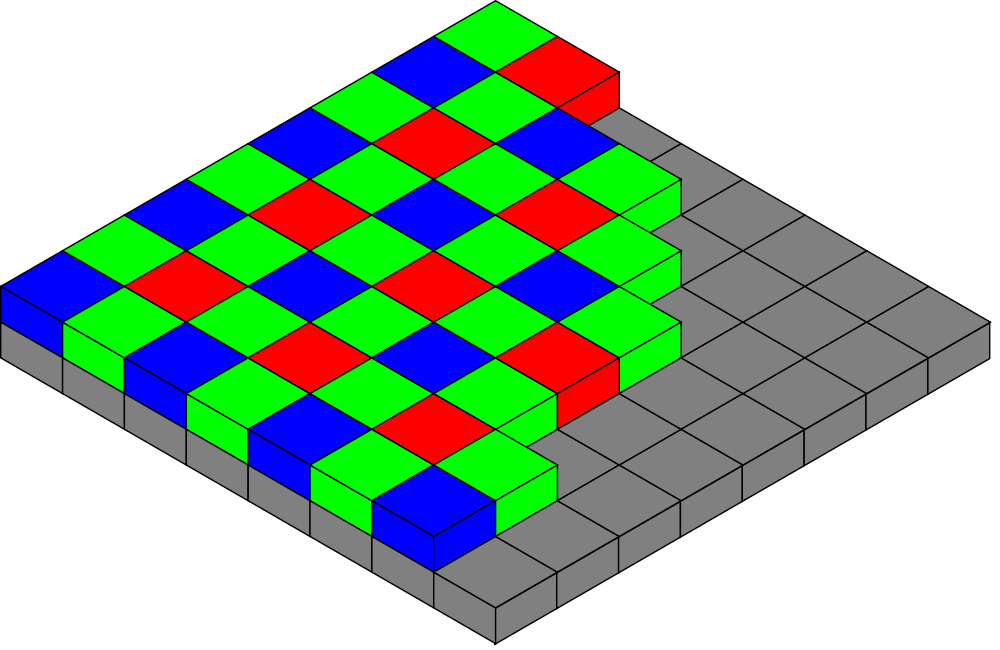
\includegraphics[width=0.4\textwidth]{images/bayer_pattern_on_sensor}
\caption{A bayer pattern on a sensor in isometric perspective \cite{img_bayer_pattern}}
\label{fig:bayer_pattern}
\end{figure}
A RGB camera is an image processing device that processes light in the visible spectrum, similar to the human eye. Modeled after the retina it has three distinct color channels - red, green and blue. There are different methods available to distinguish these channels from visible light, such as Bayer filters (Figure \ref{fig:bayer_pattern}) in front of a single sensor or using multiple sensors behind a prism.
The usage of cameras in smart environments is very common. I will present five different examples and afterwards will specify how they are linked to the properties that were defined previously.
Tabar et al. have been using a combined system of cameras, RF transmitters and wearable sensors in a home care scenario \cite{tabar2006smart}. The cameras are used to improve the accuracy of the accelerometer-based fall detection by eliminating false positives. Once a fall event occurs an algorithm tracks the posture of detected humans in the scene (Figure \ref{fig:rel_tech_body_face} - left). They used an edge detector to distinguish the human body from other objects and applied a heuristic to differentiate lying and standing.  Additionally a face detector was used to improve the recognition of human objects. Combining this with information from the fall detecting sensor and a RF based localization system they were able to achieve a good reliability in eliminating false positive alerts.
\begin{figure}[h]
\centering
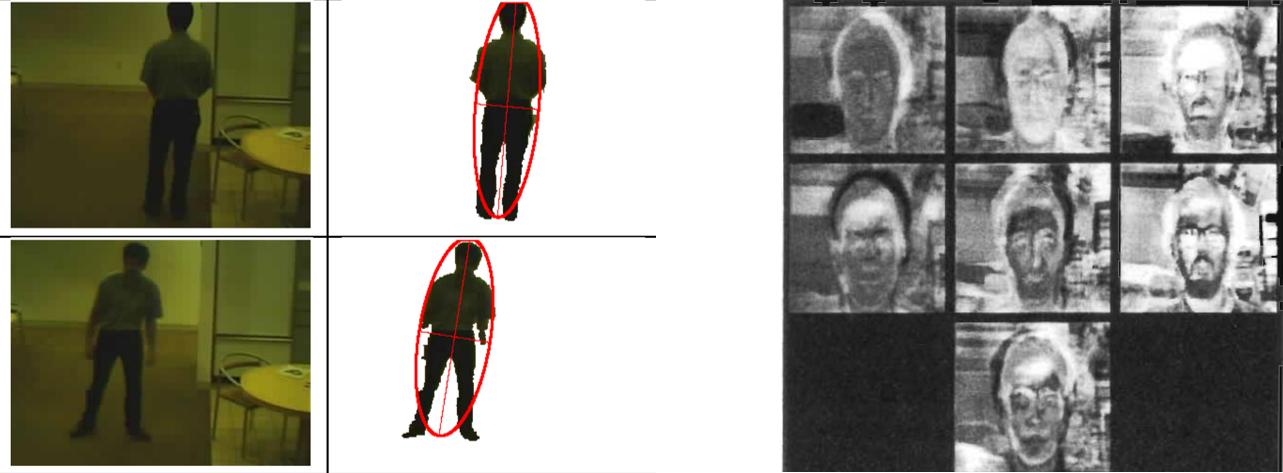
\includegraphics[width=0.9\textwidth]{images/rel_tech_body_face}
\caption{\emph{Left}: Tracking of body masks using cameras  \cite{tabar2006smart}. \emph{Right}: Eigenfaces created from input picture set \cite{pentland2000face}}
\label{fig:rel_tech_body_face}
\end{figure}

Pentland and Choudhury provided an overview of vision-based face recognition systems in the domain of smart environments \cite{pentland2000face}. The systems are able to identify users and recognize facial expressions. The proposed applications in smart environments include personalized shopping experiences based on customer recognition, behavior monitoring in child care facilities and emotion-aware systems that react to the user's current awareness. The described techniques include PCA-supported, eigenvector-based classification, face-based localization and systems based on local feature analysis (Figure \ref{fig:rel_tech_body_face} - right). Newer systems are able to operate well in unconstrained environments, that include varying expression and illumination, ageing of persons, occlusion and disguise \cite{wright2009robust}.
\begin{figure}[h]
\centering
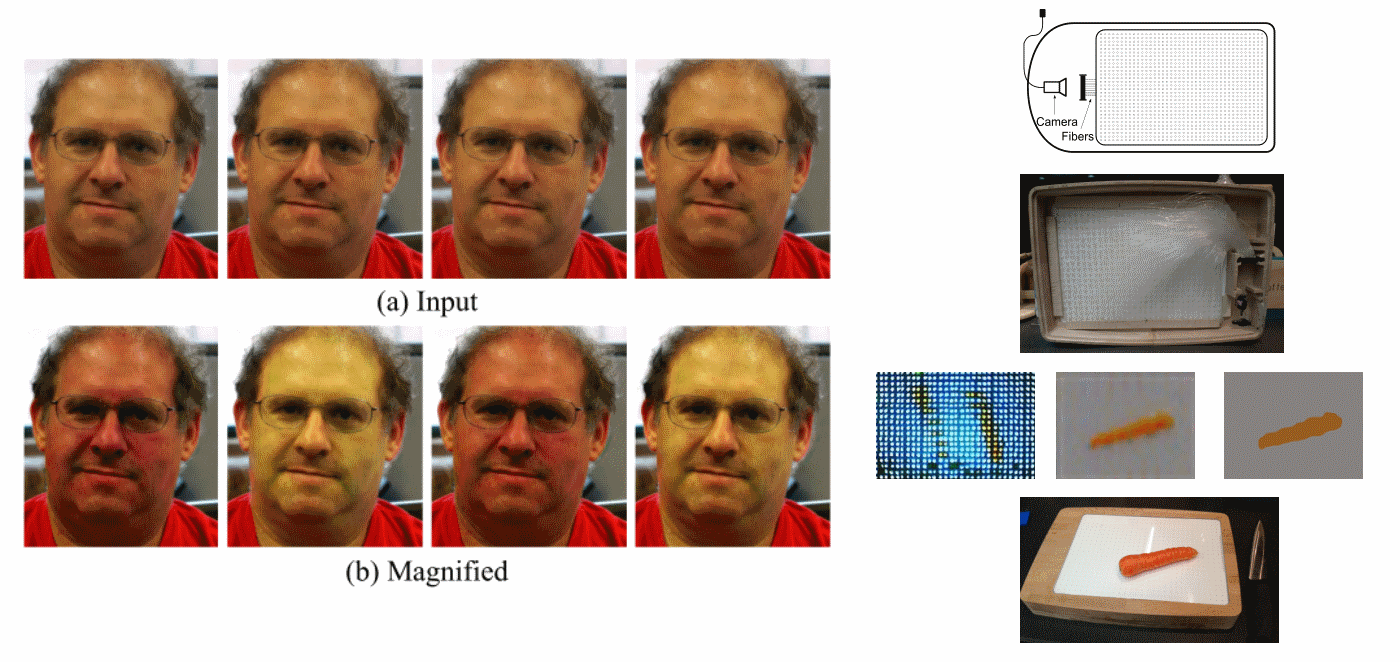
\includegraphics[width=0.7\textwidth]{images/rgb_euler_food}
\caption{\emph{Left}: Eulerian Video Magnification to attenuate the human pulse with original (a) and amplified (b) video sequence  \cite{Wu2012}. \emph{Right}: FoodBoard schematics (top), underside view (second row), original, reconstructed and segmented image (third row) and final system (bottom) \cite{pham2013foodboard}}
\label{fig:rgb_euler_food}
\end{figure}

An example for a novel image processing method that is useful in smart environments was presented by Vu et al. in 2012 \cite{Wu2012}. They are using  temporal variances of pixel values to exaggerate spatial movements and color changes that would typically be invisible to the naked eye. The method is called Eulerian Video Magnification and uses a combination of spatial decomposition and temporal filtering applied to adjacent frames. It can be tuned to different time-frequency bands to attenuate different classes of signals. Some of the proposed applications include the tracking of breathing rates of infants by attenuating chest movement, or the tracking of subtle movements, such as vibration in appliances. The example shown in Figure \ref{fig:rgb_euler_food} on the left is using a magnification of colors, in order to identify the heart rate of a person. The latter can be used for personal health applications, e.g. by integrating the system into the bath room mirror to provide an unobtrusive daily measurement and give the user feedback over a longer period of time.

A final example in this section is the FoodBoard, a smart chopping board that uses image processing to recognize the food items that are put on it \cite{pham2013foodboard}. It is shown in Figure \ref{fig:rgb_euler_food} on the right. To enable a thin footprint, ambient light is transferred to a camera using glass fibers. The picture is reconstructed and segmented, allowing to identify different items of food that are placed on it. The classification is based on a combination of Fast-Hessian and color histogram feature extractors. Pham et al. were able to distinguish 12 different ingredients with an accuracy between 59\% and 93\%. The system can be used to support dietary monitoring, give recipe guidance or support visually impaired users in identifying and tracking food.
\subsection{Infrared cameras}
\begin{figure}[h]
\centering
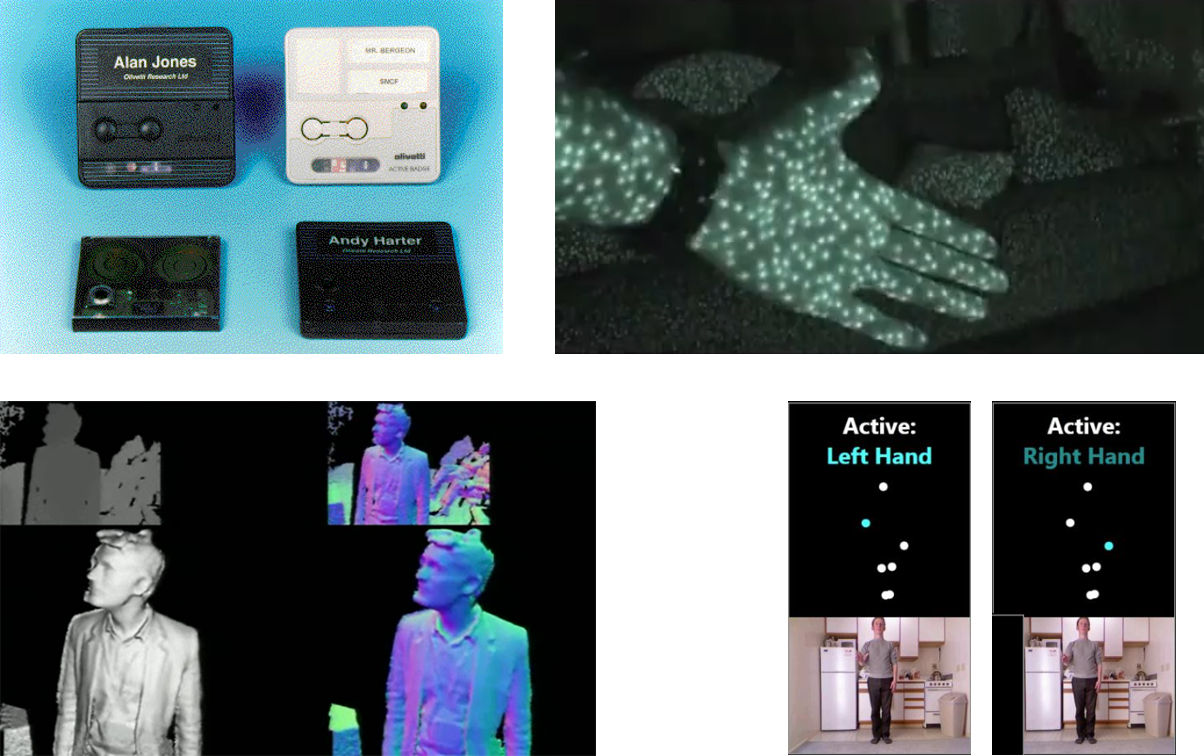
\includegraphics[width=0.9\textwidth]{images/rel_tech_infra}
\caption{\emph{Top Left}: ORL Active Badge  \cite{Weiser1991}. \emph{Top Right}: Kinect infrared projection \cite{zhang2012microsoft}. \emph{Bottom Left}: Kinect Fusion reconstrucion  \cite{Izadi2011}. \emph{Bottom Right}: Kinect kitchen interaction \cite{panger2012kinect}}
\label{fig:rel_tech_infra}
\end{figure}
Infrared imaging is using the same sensors that are suitable for visible light imaging. The difference is that they are tuned to collect electromagnetic waves of a lower wavelength that are just outside of the visible spectrum. This allows for distinct applications, such as thermal imaging, as it is possible to detect heat radiation. One of the earliest prototypes in Ubiquitous Computing designed by PARC was using the ORL Active Badge, an infrared emitter developed by Olivietti Research Laboratories that was used to identify persons operating in the environment \cite{Weiser1991} (Figure \ref{fig:rel_tech_infra} Top Left). In smart environments the most common application is using infrared cameras in combination with infrared light sources. This allows to illuminate spaces without visible artifacts to the user, thus providing imaging capabilities in dark rooms, or very specific conditions that may be required by a certain application. Another very interesting option is to use a specific projection of patterns into the scene. Analyzing the returning infrared light it is possible to infer the depth of specific pixels of the camera (Figure \ref{fig:rel_tech_infra} Top Right). This variety is called a depth camera. Particularly in the last few years the research in this domain has expanded strongly, sparked by the availability of an affordable depth camera/RGB camera combination - the Kinect by Microsoft \cite{zhang2012microsoft}. On the following pages we will present various examples of how this device can be used in smart environments to enable different applications in interaction and activity tracking.

Sung et al. have presented a system that is tracking activities of daily life based on the movements of a skeleton that is provided by the Kinect API \cite{sung2011human}. This skeleton model is based on a pose reconstruction algorithm developed by Shotton et al. \cite{Shotton2013} and is used in many different Kinect-based applications. The algorithm is using a method called hierarchical maximum entropy Markov model (MEMM). Each activity is considered to be composed of sub-activities. Based on this assumption a two-level graph is generated using dynamic programming. The system was tested with twelve activities performed in an office, a kitchen, a living room, a bathroom and a bedroom. If the person was part of the training set the precision was 84.3\% and 64.2\% for unknown persons. Some example activities of the acquired dataset are shown in Figure .

A novel method to use the Kinect for fast 3D reconstruction of scenes was presented by Izadi et al. in 2011 \cite{Izadi2011} (Figure \ref{fig:rel_tech_infra} Bottom Left). The basic premise is to use a fast registration method to combine point clouds that are generated by the system and continuously extend and optimize the current model of the scene. They are using a GPU-based ICP implementation to track the position of the camera in six degrees-of-freedom. This allows to reliably integrate the different point clouds into a single voxel grid that can be used to represent and render the scene. They proposed a number of applications ranging from phyiscal simulation of particles in the scene, to system control based on segmenting and tracking the user's hands and their interaction with arbitrary surfaces in the environment. Figure  shows some results of the touch recognition in a reconstructed scene.

Galen has presented a method to use a Kinect in a kitchen to provide touch free interaction \cite{panger2012kinect}. Two different interaction schemes are proposed. The first allows to control the applications with messy hands, the second enables to use other limbs if the hands are currently occupied (Figure \ref{fig:rel_tech_infra} Bottom Right). Three different test applications have been implemented. A recipe navigator that allows to open and navigate through different recipes. A timer that enables setting different alarm times, similar to a kitchen clock and a music player that can be controlled to choose different stations according to preference. A real life test with five subjects  did also test installation complexity, which was deemed favorable. There were some concerns in clearly distinguishing commands from random movements performed in the kitchen.

The final system based on infrared cameras is an immersive telepresence system developed by Beck et al. \cite{beck2013immersive}. Telepresence enables persons to be present as a representation in a remote place. A typical example is video conferences, but advanced system may include robotics or virtual elements. The presented system is using a single Kinect for each participant. A 3D representation is created based on the depth information of the infrared camera and on-the-fly texturing using the included RGB camera. The virtual user representations are put into a shared virutal environment and can interact with each other. Some variations were tested where local and remote users were decoupled, side-by-side or face-to-face. Different tracing and pointing gestures are supported. The supported applications included the exploration of a virtual city.

\subsection{Ultrasound sensors}
\begin{figure}[h]
\centering
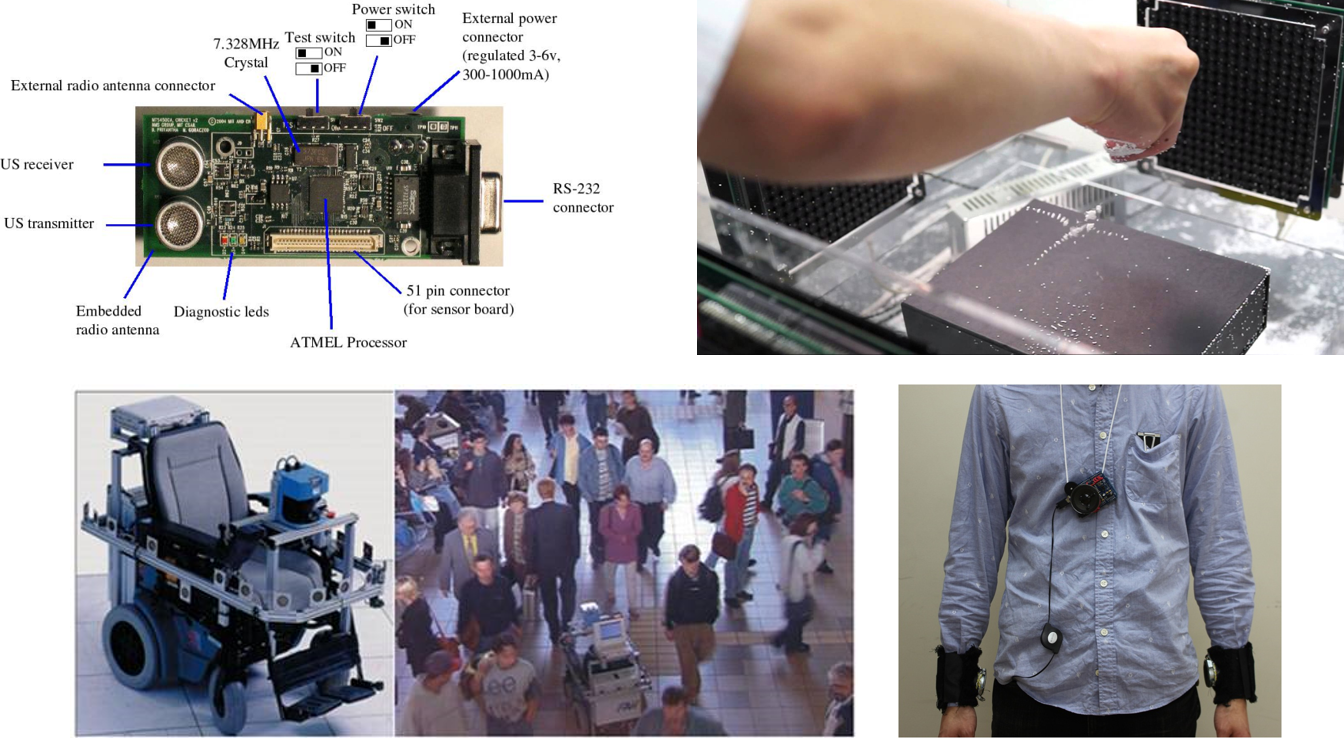
\includegraphics[width=0.9\textwidth]{images/rel_tech_ultra}
\caption{\emph{Top Left}: Cricket Indoor Localization hardware \cite{priyantha2000cricket}. \emph{Top Right}: Mid-air particle manipulation \cite{ochiai2013three}. \emph{Bottom Left}: Robotic wheelchair MAid with ultrasound range sensors \cite{prassler2001robotics}. \emph{Bottom Right}: Activity and context recognition using ultrasound sensors \cite{watanabe2013ultrasound}}
\label{fig:rel_tech_ultra}
\end{figure}
Ultrasound sensors allow detecting sound wave signals that have a frequency beyond 20kHz and are thus not audible to humans. Their propagation and reflection properties are similar to audible sound waves, thus the generated measurements can be similar. While there are natural sources of ultrasound waves the applications in smart environments do rely on active systems, that combine sound generators and sensors that measure the resulting signal. By timing the time distance between sending the signal and receiving a response it is possible to measure distances between the sender and different object.  If various receivers are used it is possible to localize the sound source, making ultrasound sensing a popular candidate in indoor localization systems. In Figure we can see a sketch of the basic functionality of ultrasound sensing systems on the left, and an example of localization using three receivers and a single source. We will present four different examples on how ultrasound sensors are used in smart environment applications.

The Cricket developed by Pryantha et al. is an example for an indoor localization system based on a badge the tracked object has to wear \cite{priyantha2000cricket}. The badge is periodically sending signals to a set of beacons that determine the distance and calculate a location. Initially it was supposed to solely rely on radiofrequency signals, but was modified to use a combination of RF and ultrasound. The rationale of this decision is the considerably slower speed of sound that simplifies measuring the time-of-flight and thus allows for more precise distance measurements. Consequently this also leads to a better precision in the localization algorithm. Additionally, the system uses some novel methods to deal with interference and multipath issues, that is dealing with reflected signals. As potential applications they propose space-dependent services that are provided as the user is identified in a certain region and guidance scenarios on a floor plan. The hardware is shown in Figure \ref{fig:rel_tech_ultra} (Top Left).

The robotic wheelchair MAid (Mobility Aid for Elderly and Disabled People) was designed to support and transport people with limited motion skills \cite{prassler2001robotics}. It is based on a commercial wheelchair that has been equipped with an intelligent control and navigation system. The system includes an ultrasound-based range finder that allows to detect obstacles in the path and circumnavigate around (Figure \ref{fig:rel_tech_ultra} Bottom Left). 

Watanabe et al. investigate the role of ultrasound sensors in recognizing activities and gestures of a user \cite{watanabe2013ultrasound}. The system is comprised of a microphone attached to a necklace and two speakers that are attached to each wrist. Based on the acquired volume and evaluation of the Doppler effect it is possible to determine both distance of the wrists from the neck and the speed of movement (Figure \ref{fig:rel_tech_ultra} Bottom Right). Watanabe et al. want to determine if this system allows for similar performance compared to other body-worn systems based on accelerometer and gyroscope data. Additionally it was evaluated if external microphones can perform as well as the neck worn microphone. The system was able to recognize 87\% of activities and gestures in a set of 10 test persons if no influencing sound was present. The ultrasound did also improve results if environmental noise was present.

A recent project at the University of Tokyo evaluates the potential of ultrasound in manipulating small particles in free-air \cite{ochiai2013three}. Using standing waves to  create sound pressure notes it is possible to apply a force to small particles that is sufficient to counteract gravity. Using a set of ultrasonic phased arrays it is possible to create these sound pressure nodes at arbitrary positions in three dimensions (Figure \ref{fig:rel_tech_ultra} Top Right). Ochiai et al. use this to move small objects around and investigate required object properties and their floating properties. So far the moved items have to be very light and smaller than 2 mm in diameter, resulting in the usage of polystyrene. The technology is also able to hold and move small amounts of fluid. Suggested applications include object manipulation in microgravity environments and projected haptic feedback systems.

\subsection{Microphone arrays}
\begin{figure}[h]
\centering
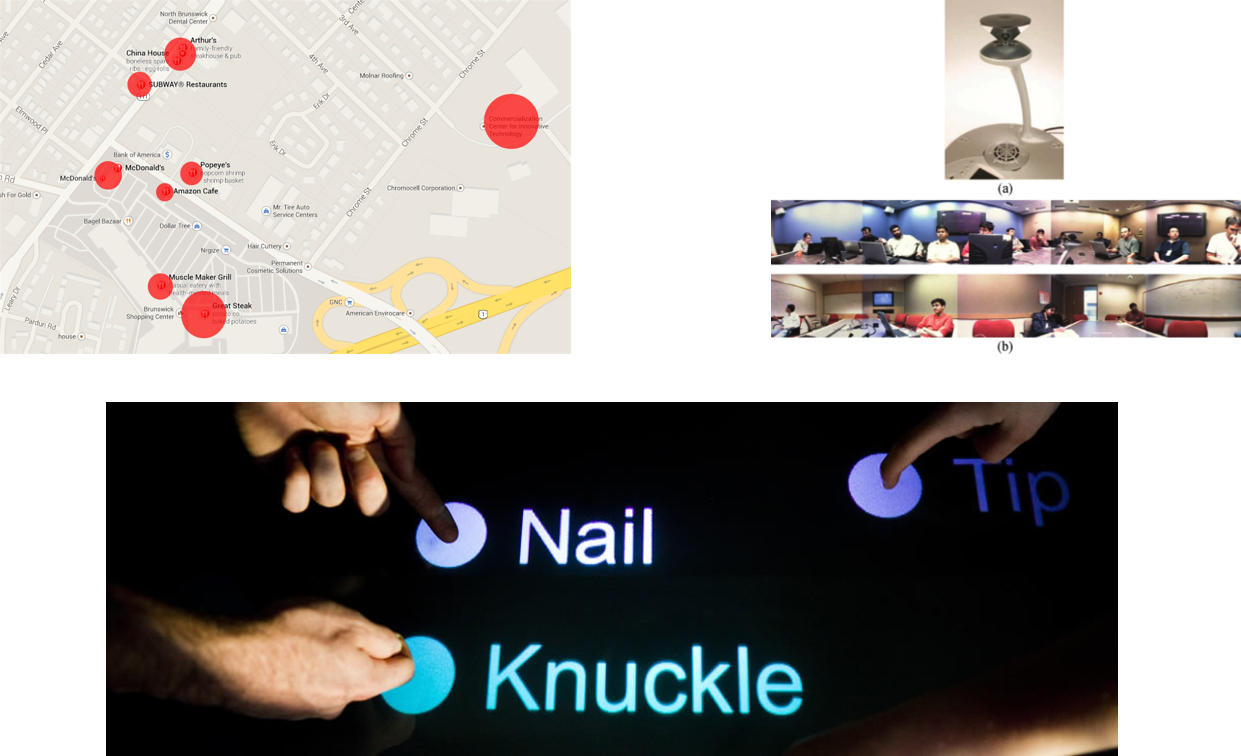
\includegraphics[width=0.9\textwidth]{images/rel_tech_mic}
\caption{\emph{Top Left}: Visualization of speaker count in different areas \cite{xu2013crowd++}. \emph{Top Right}: Directional microphone and conference room for speech source localization \cite{zhang2008maximum}. \emph{Bottom}: TapSense detecting different tap events \cite{harrison2011tapsense}.}
\label{fig:rel_tech_mic}
\end{figure}
Microphones are signal receivers that are tuned to detect sound frequency ranges that are audible by humans. Typically they consist of a piezo element that transfers vibration to an electric current that is amplified. Most human activities produce some kind of sound. As opposed to the presented ultrasound system, microphones typically operate passive. That is there is usually no dedicated signal source, but instead naturally occurring sounds are picked up. By combining microphones or arrays thereof with data processing systems that are aimed at analyzing specific sound patterns we are able to get feedback on human activities. Looking at smart environments there are numerous use cases that can benefit from microphones as sensors. In this section we will present four different systems that cover a large variety of different applications, ranging from breathing rate detection to estimating the number of speakers in large groups.

Detecting the breathing pattern of a person has several applications in smart environments. Apart from medical applications that require detecting abnormal breathing in risk groups it is also possible to track training progress using such a system or provide a measure for the current attention level in affective computing. Corbishley et al. investigated using very small microphones in mobile devices to enable detecting the breathing rate \cite{corbishley2008breathing}. The algorithm is designed to be applicable on single ICs, allowing for miniaturization and energy efficiency. Even with the presence of noise the combined score for true negatives and true positives was as high as 91.3\%. Using small and energy efficient systems also enables unobtrusive applications in non-mobile environments, e.g. placing such a system close to the bed to detect the breathing rate while the user is sleeping.

Collaborative applications are an important aspect of smart environments, e.g. to link together meeting places at different places, similar to the presented telepresence applications. If a multitude of speakers is present it gets increasingly difficult to provide a system that enables proper speech transmission for all participants. Using an array of microphones it is possible to focus the attention on the person currently speaking and filter out environmental noise. A project at Microsoft Research investigated using a maximum likelihood of two known techniques, beamforming and speech source localization, to enable a reliable speaker selection \cite{zhang2008maximum} (Figure \ref{fig:rel_tech_mic} - Top Right). Additionally the framework enables a good adaptation even if directional microphones are used that are placed close to each other. The method provides a real life accuracy of more than 90\%.

A fairly new work was performed by Xu et al. \cite{xu2013crowd++}, called Crowd++. Their idea is to use smartphone microphones to identify the number of speakers in crowded environments. Such system could be used to estimate the number of persons in a given place and potentially react quickly if a crowd panic may occur. The method is based on an unsupervised machine learning classification of short audio parts that are picked up by the individual microphones in the handsets. It was tested by 120 participants in 10 different environments and allowed detecting the number of persons with an average error of 1.5 persons (Figure \ref{fig:rel_tech_mic} - Top Left). No dedicated hardware is required to achieve this precision, enabling an application using off-the-shelf smartphones.

Microphones can also be used to analyze the mechanical surface waves that occur when objects interact with each other. Harrison et al. have designed TapSense, a microphone based sensor system that improves touch interaction by classifying the sounds created by different objects hitting the surface \cite{harrison2011tapsense}. In particular different parts of the hand can be distinguished, including nail, knuckle or tip. Potential applications are improving touch interaction on touch screens by enabling different forms of interaction, but also can be adapted to mobile devices, that typically have less interaction space and increase the expressiveness of different touch gestures. The achievable accuracy was between 95\% using four different input types up to 99\% when using just two input sets, such as finger and pen (Figure \ref{fig:rel_tech_mic} - Bottom).

\subsection{Radiofrequency sensing}
\begin{figure}[h]
\centering
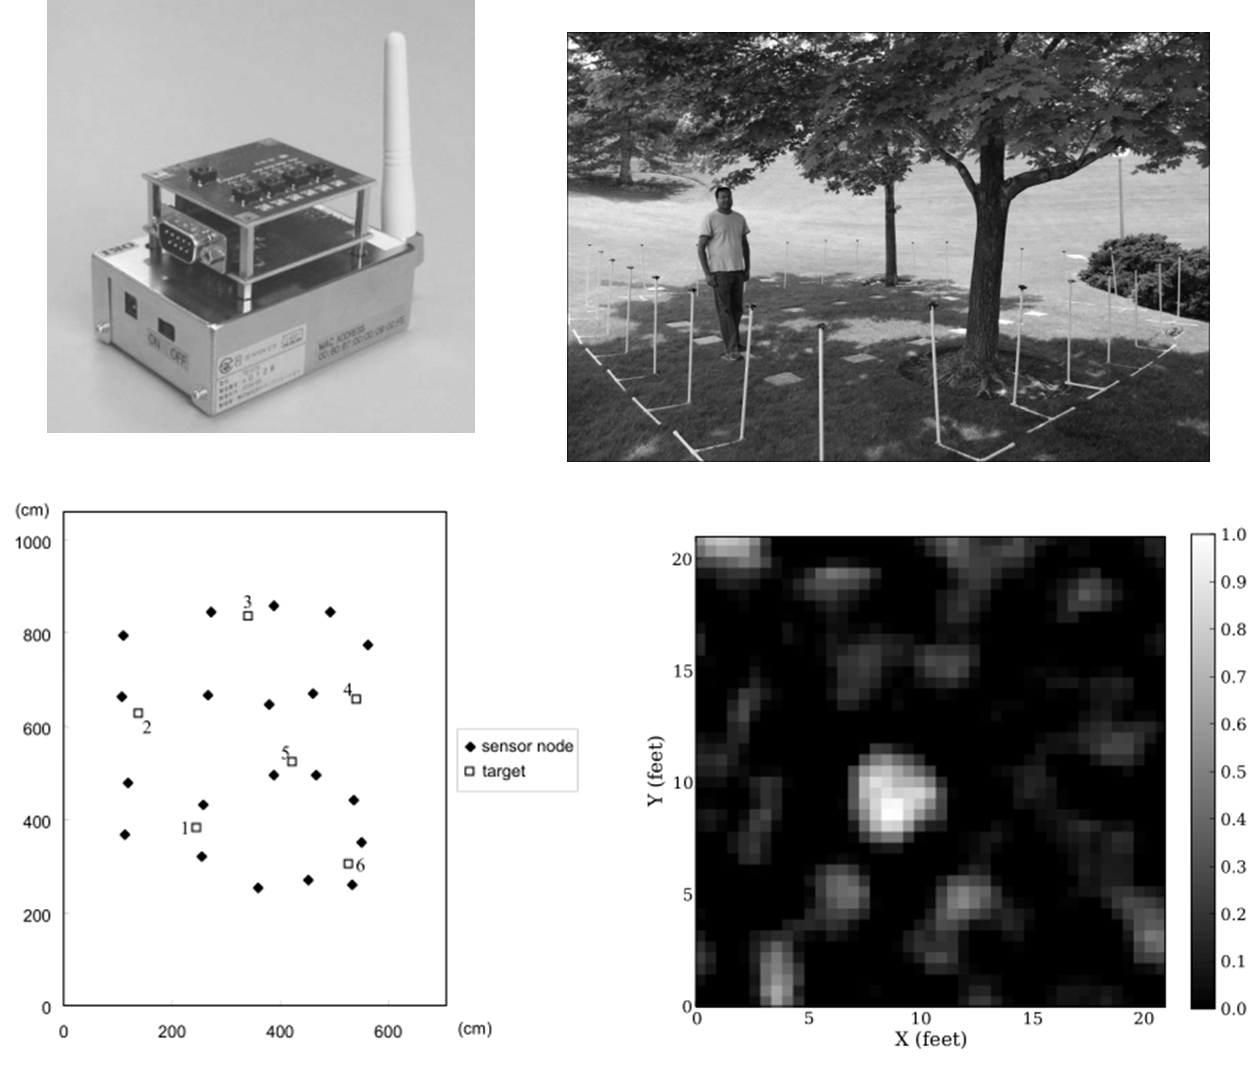
\includegraphics[width=0.9\textwidth]{images/tech_mic1}
\caption{\emph{Top left} ZigBee node. \emph{Bottom Left} Sensors and targets in larger room \cite{sugano2006indoor}. \emph{Top right} Photo of radio tomography setup. \emph{Bottom right} Result attenuated signal \cite{wilson2010radio}.}
\label{fig:tech_mic1}
\end{figure}

Radiofrequency sensing is a traditional field for sensors. Radar is a system that uses radio waves to acquire direction, speed, distance or altitude of objects and was developed at the beginning of World War II. This variety is using active sensing and emits radio waves that are reflected by objects. Most applications in smart environments similarly rely on active systems. A popular signal source are WiFi signals, intended to wirelessly transmit information between several systems. The systems are wide-spread, with all smartphones possesing two or more wireless technologies (typically 4G/3G/GSM for long range communication, WLAN for medium range communication and Bluetooth/NFC for short range communication) that can be used in coordination with stations placed in the environment. The signal processing of the wireless LAN sets generates some additional data that can be used, most notably the signal strength (RSSI). We will present different systems that show some different ways how radiofrequency sensing can be used in smart environments.

Radiofrequency based systems are very popular for indoor localization applications. We previously glimpsed at the difficulty of time-of-flight systems in the electromagnetic specturm. Thus most systems rely on a different approach, using the received signal strength (RSSI). If the initial signal strength is known and we have a good estimate how the signal propagates we can estimate the loss of signal strength at a certain distance. An accepted work that helped shaping this domain is the system created by Sugano et al. in 2006 that uses a ZigBee-based network with a limited number of nodes receiving RSSI information \cite{sugano2006indoor}. Based on this it is possible to locate one or more users with an error between 1.5-2m. This often is sufficient to distinguish the room a person is currently in, enabling a room-based system adaptation, which is suitable for many applications. A photo of a ZigBee node and results in a larger conference room are shown in Figure \ref{fig:tech_mic1} on the left.

A different approach for RSSI based systems was presented by Wilson and Patwari in 2010 \cite{wilson2010radio}. They are using tomography methods to determine the location of users. By placing a large number of sensors on the outer limits of the environment and creating a unique link between each, it is possible to infer the position based on the signal attenuation when a person moves in the environment. The human body absorbs some of the signal, resulting in a reduced received RSSI in the affected nodes. The error for standing persons was between 0.64cm for a single person and 1.10cm for two persons. An image of the test area and the resulting reconstructed attenuation map are shown in Figure \ref{fig:tech_mic1} on the right.

\begin{figure}[h]
\centering
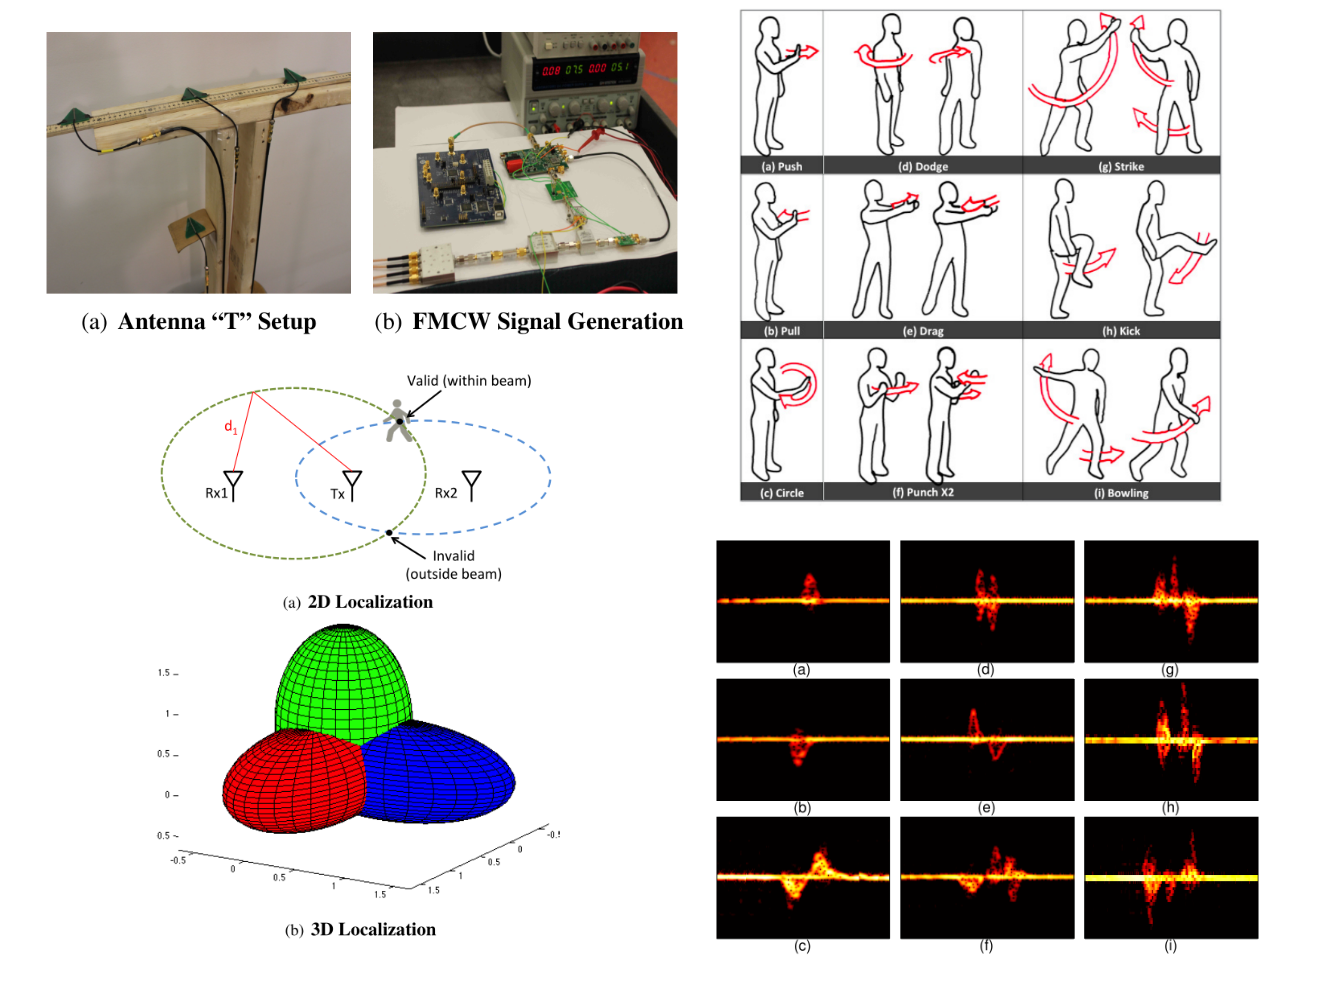
\includegraphics[width=0.9\textwidth]{images/tech_mic2}
\caption{\emph{Top left} WiTrack antennas and signal generator. \emph{Bottom Left} WiTrack 2D and 3D localization method \cite{adib20133d}. \emph{Top right} WiSee supported gestures. \emph{Bottom right} WiSee Doppler profiles of gestures \cite{pu2013whole}.}
\label{fig:tech_mic2}
\end{figure}

A final system that provides a localization is WiTrack, presented by Adib et al in 2013 \cite{adib20133d}. It uses the signal reflected by the human body to provide a location estimate based on time-of-flight. As mentioned previously this is challenging due to the propagation speed within the electromagnetic field. To overcome this issue they are using a method called frequency modulated carrier wave that transfers time differences to the frequency domain. Looking at the spectrum of received signal these shifts can be analyzed. The resulting location has an accuracy of 10-13 cm in x and y and 21 cm in z dimension. Additional use cases are provided in determining coarse arm or foot gestures and enabling an accurate detection of falls of a person. Some limitations of this approach include a restriction to just one person and that the tracked object has to move. In Figure \ref{fig:tech_mic2} on the left we can see pictures of the antenna setup, the signal generator and how the location is determined in two and three dimensions.

The final radiofrequency system I want to present is WiSee, developed at the University of Washington by Pu et al. \cite{pu2013whole}. They are using Wi-Fi to enable gesture recognition in large areas without requiring a line-of-sight. They are analyzing the Doppler shift resulting from human activity in order to classify different gestures. They are using MIMO (multiple input multiple output) to distinguish between non-interacting persons in the environment and the person performing gestures. To equip a whole appartment only a single receiver and two transmitters are necessary. The achievable accuracy varies according to persons present and number/type of devices involved but peaks at an accuracy of 94\% for detecting nine different whole body gestures. The supported gestures and their Doppler profiles are shown in Figure \ref{fig:tech_mic2} on the right.
\section{Applications in smart environments}
The field of smart environments is not strictly and conclusively limited and distinguished from other fields in technology, using influences from disciplines including electric engineering, behavioral psychology, computer science or mechanical engineering. Accordingly, it is difficult to formally list or distinguish all applications that are relevant or have been tackled in previous work. Thus, I will refer to previous collections of surveys, books and state-of-the-art in the associated disciplines smart environments, ambient intelligence and ubiquitous computing to get an informed selection of relevant applications that could potentially be supported by capacitive proximity sensors. The chosen collections of applications are taken from Cook et al. that presented a survey on recent developments in smart environments research in 2007 \cite{cook2007smart}. Augusto et al. edited a book on ambient intelligence in 2009, including chapters on various domains and applications. The final source is the book \emph{Ubiquitous Computing} by Poslad, released in 2011 \cite{poslad2011ubiquitous}.

The applications presented in those works are analyzed and grouped into a limited set of higher level applications. With this grouping I have tried to emphasize the technological similarities of the different applications in preparation for the later benchmarking process. The results can be found in Table . On the following pages the different groups will be introduced with some examples and specific information on the sensor measurements that are required. The determined groups are the basis for further references to different use cases and will be referred to throughout this work.
\subsection{Localization}
\subsection{Activity Recognition}
\subsection{Smart Appliances}
\subsection{Human-Computer Interaction}
\subsection{Physiological Sensing}
\subsection{Augmented and Virtual Reality}



